\part{Programming Techniques}\label{programming-techniques.part}


\chapter{Reparameterization \& Change of Variables}\label{change-of-variables.chapter}

\noindent
As with BUGS, Stan supports a direct encoding of reparameterizations.
Stan also supports changes of variables by directly incrementing the
log probability accumulator with the log Jacobian of the transform.

\section{Theoretical and Practical Background}

A Bayesian posterior is technically a probability \emph{measure},
which is a parameterization-invariant, abstract mathematical object.%
%
\footnote{This is in contrast to (penalized) maximum likelihood
  estimates, which are not parameterization invariant.}
%
Stan's modeling language, on the other hand, defines a probability
\emph{density}, which is a non-unique, parameterization-dependent
function in $\reals^N \rightarrow \reals^{+}$.  In practice, this
means a given model can be represented different ways in Stan, and
different representations have different computational performances.

As pointed out by \cite{Gelman:2004} in a paper discussing the
relation between parameterizations and Bayesian modeling, a change of
parameterization often carries with it suggestions of how the model
might change, because we tend to use certain natural classes of prior
distributions.  Thus, it's not \emph{just}\ that we have a fixed
distribution that we want to sample from, with reparameterizations
being computational aids.  In addition, once we reparameterize and add
prior information, the model itself typically changes, often in useful
ways.%
%
\footnote{Gelman's handy statistical lexicon
  (\url{http://andrewgelman.com/2009/05/24/handy_statistic/}) calls
  this \emph{The Pinocchio Principle}, ``A model that is created
  solely for computational reasons can take on a life of its own.''
  This principle is also related to what Gelman calls \emph{The Folk
    Theorem}, ``When you have computational problems, often there's a
  problem with your model.''}




\section{Reparameterizations}

Reparameterizations may be implemented directly using the transformed
parameters block or just in the model block.

\subsection{Beta and Dirichlet Priors}

The beta and Dirichlet distributions may both be reparameterized from
a vector of counts to use a mean and total count.

\subsubsection{Beta Distribution}

For example, the Beta distribution is parameterized by two positive
count parameters $\alpha, \beta > 0$.  The following example
illustrates a hierarchical Stan model with a vector of parameters
\code{theta} are drawn i.i.d.\ for a Beta distribution whose
parameters are themselves drawn from a hyperprior distribution.
%
\begin{stancode}
parameters {
  real<lower = 0> alpha;
  real<lower = 0> beta;
  ...
model {
  alpha ~ ...
  beta ~ ...
  for (n in 1:N)
    theta[n] ~ beta(alpha, beta);
  ...
\end{stancode}

It is often more natural to specify hyperpriors in terms of
transformed parameters.  In the case of the Beta, the obvious choice
for reparameterization is in terms of a mean parameter
\[
\phi = \alpha / (\alpha + \beta)
\]
and total count parameter
\[
\lambda = \alpha + \beta.
\]
Following \citep[Chapter 5]{GelmanEtAl:2013}, the mean
gets a uniform prior and the count parameter a Pareto prior with
$p(\lambda) \propto \lambda^{-2.5}$.
%
\begin{stancode}
parameters {
  real<lower=0,upper=1> phi;
  real<lower=0.1> lambda;
  ...
transformed parameters {
  real<lower=0> alpha = lambda * phi;
  real<lower=0> beta = lambda * (1 - phi);
  ...
model {
  phi ~ beta(1, 1); // uniform on phi, could drop
  lambda ~ pareto(0.1, 1.5);
  for (n in 1:N)
    theta[n] ~ beta(alpha, beta);
  ...
\end{stancode}
%
The new parameters, \code{phi} and \code{lambda}, are declared in the
parameters block and the parameters for the Beta distribution,
\code{alpha} and \code{beta}, are declared and defined in the
transformed parameters block.  And If their values are not of interest,
they could instead be defined as local variables in the model as
follows.
%
\begin{stancode}
model {
  real alpha = lambda * phi
  real beta = lambda * (1 - phi);
...
  for (n in 1:N)
    theta[n] ~ beta(alpha, beta);
...
}
\end{stancode}
%
With vectorization, this could be expressed more compactly and
efficiently as follows.
\begin{stancode}
model {
  theta ~ beta(lambda * phi, lambda * (1 - phi));
...
}
\end{stancode}
%
If the variables \code{alpha} and \code{beta} are of interest, they
can be defined in the transformed parameter block and then used in the
model.


\subsubsection{Jacobians not Necessary}

Because the transformed parameters are being used, rather than given a
distribution, there is no need to apply a Jacobian adjustment for the
transform.  For example, in the beta distribution example,
\code{alpha} and \code{beta} have the correct posterior distribution.

\subsubsection{Dirichlet Priors}

The same thing can be done with a Dirichlet, replacing the mean for
the Beta, which is a probability value, with a simplex.  Assume there
are $K > 0$ dimensions being considered ($K=1$ is trivial and $K=2$
reduces to the beta distribution case).  The traditional prior is
%
\begin{stancode}
parameters {
  vector[K] alpha;
  simplex[K] theta[N];
  ...
model {
  alpha ~ ...;
  for (n in 1:N)
    theta[n] ~ dirichlet(alpha);
}
\end{stancode}
%
This provides essentially $K$ degrees of freedom, one for each
dimension of \code{alpha}, and it is not obvious how to specify a
reasonable prior for \code{alpha}.

An alternative coding is to use the mean, which is a simplex, and a
total count.
%
\begin{stancode}
parameters {
  simplex[K] phi;
  real<lower=0> kappa;
  simplex[K] theta[N];
  ...
transformed parameters {
  vector[K] alpha = kappa * phi;
  ...
}
model {
  phi ~ ...;
  kappa ~ ...;
  for (n in 1:N)
    theta[n] ~ dirichlet(alpha);
\end{stancode}
%
Now it is much easier to formulate priors, because \code{phi} is the
expected value of \code{theta} and \code{kappa} (minus \code{K}) is
the strength of the prior mean measured in number of prior observations.

\subsection{Transforming Unconstrained Priors: Probit and Logit}

If the variable $u$ has a  distribution, then
$\mbox{logit}(u)$ is distributed as $\distro{Logistic}(0, 1)$.  This
is because inverse logit is the cumulative distribution function (cdf)
for the logistic distribution, so that the logit function itself is
the inverse cdf and thus maps a uniform draw in $(0, 1)$ to a
logistically-distributed quantity.

Things work the same way for the probit case: if $u$ has a
$\distro{Uniform}(0, 1)$ distribution, then $\Phi^{-1}(u)$ has a
$\distro{Normal}(0, 1)$ distribution.  The other way around, if $v$
has a $\distro{Normal}(0, 1)$ distribution, then $\Phi(v)$ has a
$\distro{Uniform}(0, 1)$ distribution.

In order to use the probit and logistic as priors on variables
constrained to $(0, 1)$, create an unconstrained variable and
transform it appropriately.  For comparison, the following Stan
program fragment declares a $(0, 1)$-constrained parameter
\code{theta} and gives it a beta prior, then uses it as a parameter in
a distribution (here using \code{foo} as a placeholder).
%
\begin{stancode}
parameters {
  real<lower = 0, upper = 1> theta;
...
model {
  theta ~ beta(a, b);
  ...
  y ~ foo(theta);
...
\end{stancode}
%
If the variables \code{a} and \code{b} are one, then this imposes
a uniform distribution \code{theta}.  If \code{a} and \code{b} are
both less than one, then the density on \code{theta} has a U shape,
whereas if they are both greater than one, the density of \code{theta}
has an inverted-U or more bell-like shape.

Roughly the same result can be achieved with unbounded parameters that
are probit or inverse-logit-transformed.  For example,
%
\begin{stancode}
parameters {
  real theta_raw;
...
transformed parameters {
  real<lower = 0, upper = 1> theta = inv_logit(theta_raw);
...
model {
  theta_raw ~ logistic(mu, sigma);
  ...
  y ~ foo(theta);
...
\end{stancode}
%
In this model, an unconstrained parameter \code{theta\_raw} gets a
logistic prior, and then the transformed parameter \code{theta} is
defined to be the inverse logit of \code{theta\_raw}.  In this
parameterization, \code{inv\_logit(mu)} is the mean of the implied
prior on \code{theta}.  The prior distribution on \code{theta} will be
flat if \code{sigma} is one and \code{mu} is zero, and will be
U-shaped if \code{sigma} is larger than one and bell shaped if
\code{sigma} is less than one.

When moving from a variable in $(0, 1)$ to a simplex, the same trick
may be performed using the softmax function, which is a multinomial
generalization of the inverse logit function.  First, consider a
simplex parameter with a Dirichlet prior.
%
\begin{stancode}
parameters {
  simplex[K] theta;
...
model {
  theta ~ dirichlet(a);
  ...
  y ~ foo(theta);
\end{stancode}
%
Now \code{a} is a vector with \code{K} rows, but it has the same shape
properties as the pair \code{a} and \code{b} for a beta; the beta
distribution is just the distribution of the first component of a
Dirichlet with parameter vector $[a b]^{\top}$.  To formulate an
unconstrained prior, the exact same strategy works as for the beta.
%
\begin{stancode}
parameters {
  vector[K] theta_raw;
...
transformed parameters {
  simplex[K] theta = softmax(theta_raw);
...
model {
  theta_raw ~ multi_normal_cholesky(mu, L_Sigma);
\end{stancode}
%
The multivariate normal is used for convenience and efficiency with
its Cholesky-factor parameterization.  Now the mean is controlled by
\code{softmax(mu)}, but we have additional control of covariance
through \code{L\_Sigma} at the expense of having on the order of $K^2$
parameters in the prior rather than order $K$.  If no covariance is
desired, the number of parameters can be reduced back to $K$ using a
vectorized normal distribution as follows.
%
\begin{stancode}
  theta_raw ~ normal(mu, sigma);
\end{stancode}
%
where either or both of \code{mu} and \code{sigma} can be vectors.


% \subsection{Transforming multinomial to Poisson}

% Lancaster \cite{lancaster:2000} provides an efficient
% reparameterization of the multinomial distribution in terms of the
% Poisson distribution.  Suppose we have a multinomial such as the
% following:

% \begin{stancode}
% data {
%   int<lower = 0> K;        // number of categories
%   int<lower = 0> x[N, K];  // outcomes
% \end{stancode}


% This reparameterization is critical for
% applying multinomials efficiently in Stan.

% \begin{stancode}
% data {
%   int<lower = 0> K;  // number of categories
%   ...
% }
% parameters {
%   vector[K] log_alpha_star;
%   ...
% }
% transformed parameters {
%   vecotr[K] log_alpha;
%   for (g in 1:groups)
%     log_alpha[g] = log_alphastar[g] - log_sum_exp(x[g] * beta);
% }
% model {
%   log_alpha_star ~ ...;  // some prior
%   x ~ poisson_log(log_alpha);
% }
% \end{stancode}





\section{Changes of Variables}

Changes of variables are applied when the transformation of a
parameter is characterized by a distribution.  The standard textbook
example is the lognormal distribution, which is the distribution of a
variable $y > 0$ whose logarithm $\log y$ has a normal distribution.
Note that the distribution is being assigned to $\log y$.

The change of variables requires an adjustment to the probability to
account for the distortion caused by the transform.  For this to work,
univariate changes of variables must be monotonic and differentiable
everywhere in their support.

For univariate changes of variables, the resulting probability must be
scaled by the absolute derivative of the transform (see
\refsection{change-of-variables} for more precise definitions of
univariate changes of variables).

In the case of log normals, if $y$'s logarithm is normal with mean
$\mu$ and deviation $\sigma$, then the distribution of $y$ is given by
\[
p(y)
\ = \
\distro{Normal}(\log y| \mu, \sigma) \  \left| \frac{d}{dy} \log y \right|
\ = \
\distro{Normal}(\log y| \mu, \sigma) \frac{1}{y}.
\]
Stan works on the log scale to prevent underflow, where
\[
\log p(y)
=
\log \distro{Normal}(\log y| \mu, \sigma)
- \log y.
\]

In Stan, the change of variables can be applied in the sampling
statement.  To adjust for the curvature, the log probability
accumulator is incremented with the log absolute derivative of the
transform.  The lognormal distribution can thus be implemented
directly in Stan as follows.%
%
\footnote{This example is for illustrative purposes only; the
  recommended way to implement the lognormal distribution in Stan is
  with the built-in \code{lognormal} probability function (see \refsection{lognormal}).}
%
\begin{stancode}
parameters {
  real<lower=0> y;
  ...
model {
  log(y) ~ normal(mu, sigma);
  target += -log(y);
  ...
\end{stancode}
%
It is important, as always, to declare appropriate constraints on
parameters;  here \code{y} is constrained to be positive.

It would be slightly more efficient to define a local variable for the
logarithm, as follows.
%
\begin{stancode}
model {
  real log_y;
  log_y = log(y);
  log_y ~ normal(mu, sigma);
  target += -log_y;
  ...
\end{stancode}
%

If \code{y} were declared as data instead of as a parameter, then the
adjustment can be ignored because the data will be constant and Stan
only requires the log probability up to a constant.

\subsection{Change of Variables vs.\ Transformations}

This section illustrates the difference between a change of variables
and a simple variable transformation.  A transformation samples a
parameter, then transforms it, whereas a change of variables
transforms a parameter, then samples it.  Only the latter requires a
Jacobian adjustment.

Note that it does not matter whether the probability function is
expressed using a sampling statement, such as
%
\begin{stancode}
log(y) ~ normal(mu, sigma);
\end{stancode}
%
or as an increment to the log probability function, as in
%
\begin{stancode}
target += normal_lpmf(log(y) | mu, sigma);
\end{stancode}

\subsubsection{Gamma and Inverse Gamma Distribution}\label{jacobian-adjustment.section}

Like the log normal, the inverse gamma distribution is a distribution
of variables whose inverse has a gamma distribution.  This section
contrasts two approaches, first with a transform, then with a change
of variables.

The transform based approach to sampling \code{y\_inv} with an inverse
gamma distribution can be coded as follows.
%
\begin{stancode}
parameters {
  real<lower=0> y;
}
transformed parameters {
  real<lower=0> y_inv;
  y_inv = 1 / y;
}
model {
  y ~ gamma(2,4);
}
\end{stancode}
%
The change-of-variables approach to sampling \code{y\_inv} with an
inverse gamma distribution can be coded as follows.
%
\begin{stancode}
parameters {
  real<lower=0> y_inv;
}
transformed parameters {
  real<lower=0> y;
  y = 1 / y_inv;  // change variables
}
model {
  y ~ gamma(2,4);
  target +=  -2 * log(y_inv);  //  Jacobian adjustment;
}
\end{stancode}
%
The Jacobian adjustment is the log of the absolute derivative of the
transform, which in this case is
%
\[
\log \left| \frac{d}{du} \left( \frac{1}{u} \right) \right|
\ = \
\log | - u^{-2} |
\ = \
\log u^{-2}
\ = \
 -2 \log u.
\]


\subsection{Multivariate Changes of Variables}

In the case of a multivariate transform, the log of the Jacobian of
the transform must be added to the log probability accumulator (see
the subsection of \refsection{change-of-variables} on multivariate
changes of variables for more precise definitions of multivariate
transforms and Jacobians).  In Stan, this can be coded as follows in
the general case where the Jacobian is not a full matrix.
%
\begin{stancode}
parameters {
  vector[K] u;      // multivariate parameter
   ...
transformed parameters {
  vector[K] v;     // transformed parameter
  matrix[K, K] J;   // Jacobian matrix of transform
  ... compute v as a function of u ...
  ... compute J[m, n] = d.v[m] / d.u[n] ...
  target += log(fabs(determinant(J)));
  ...
model {
  v ~ ...;
  ...
\end{stancode}
%
Of course, if the Jacobian is known analytically, it will be more
efficient to apply it directly than to call the determinant function,
which is neither efficient nor particularly stable numerically.

In many cases, the Jacobian matrix will be triangular, so that only
the diagonal elements will be required for the determinant
calculation.  Triangular Jacobians arise when each element \code{v[k]}
of the transformed parameter vector only depends on elements
\code{u[1]}, \ldots, \code{u[k]} of the parameter vector.  For
triangular matrices, the determinant is the product of the diagonal
elements, so the transformed parameters block of the above model can
be simplified and made more efficient by recoding as follows.
%
\begin{stancode}
transformed parameters {
  ...
  vector[K] J_diag;  // diagonals of Jacobian matrix
  ...
  ... compute J[k, k] = d.v[k] / d.u[k] ...
  target += sum(log(J_diag));
  ...
\end{stancode}


\section{Vectors with Varying Bounds}

Stan only allows a single lower and upper bound to be declared in the
constraints for a container data type.  But suppose we have a vector
of parameters and a vector of lower bounds?  Then the transforms and
Jacobians (all of which are described in
\refchapter{variable-transforms}) have to be calculated in Stan.

\subsection{Varying Lower Bounds}

For example, suppose there is a vector parameter $\alpha$ with a
vector $L$ of lower bounds.  The simplest way to deal with this if $L$
is a constant is to shift a lower-bounded parameter.
%
\begin{stancode}
data {
  int N;
  vector[N] L;  // lower bounds
  ...
parameters {
  vector<lower=0>[N] alpha_raw;
  ...
transformed parameters {
  vector[N] alpha = L + alpha_raw;
  ...
\end{stancode}
%
The Jacobian for adding a constant is one, so its log drops out of the
log density.

Even if the lower bound is a parameter rather than data, there is no
Jacobian required, because the transform from $(L, \alpha_{\mathrm
  raw})$ to $(L + \alpha_{\mathrm raw}, \alpha_{\mathrm raw}$ produces
a Jacobian derivative matrix with a unit determinant.

It's also possible implement the transform by directly transforming
an unconstrained parameter and accounting for the Jacobian.
%
\begin{stancode}
data {
  int N;
  vector[N] L;  // lower bounds
  ...
parameters {
  vector[N] alpha_raw;
  ...
transformed parameters {
  vector[N] alpha;
  alpha = L + exp(my_vec_raw);
  ...
model {
  target += sum(alpha_raw);  // log Jacobian
  ...
\end{stancode}
%
The adjustment in the the log Jacobian determinant of the transform
mapping $\alpha_{\mathrm{raw}}$ to $\alpha = L +
\exp(\alpha_{\mathrm{raw}})$.  The details are simple in this case
because the Jacobian is diagonal; see
\refsection{lower-bound-transform} for details.  Here $L$ can even be
a vector containing parameters that don't depend on
$\alpha_{\mathrm{raw}}$; if the bounds do depend on
$\alpha_{\mathrm{raw}}$ then a revised Jacobian needs to be calculated
taking into account the dependencies.

\subsection{Varying Upper and Lower Bounds}

Suppose there are lower and upper bounds that vary by parameter.
These can be applied to shift and rescale a parameter constrained to
$(0, 1)$.
%
\begin{stancode}
data {
  int N;
  vector[N] L;  // lower bounds
  vector[N] U;  // upper bounds
  ...
parameters {
  vector<lower=0, upper=1>[N] alpha_raw;
  ...
transformed parameters {
  vector[N] alpha = L + (U - L) .* alpha_raw;
\end{stancode}
%
The expression \code{U - L} is multiplied by \code{alpha\_raw}
elementwise to produce a vector of variables in $(0, U-L)$, then
adding $L$ results in a variable ranging between $(L, U)$.

In this case, it is important that $L$ and $U$ are constants,
otherwise a Jacobian would be required when multiplying by $U - L$.



\chapter{Custom Probability Functions}%
\label{custom-probability-functions.chapter}

\noindent
Custom distributions may also be implemented directly within Stan's
programming language.  The only thing that is needed is to increment
the total log probability.  The rest of the chapter provides two
examples.

\section{Examples}

\subsection{Triangle distribution}

A simple example is the triangle distribution,
whose density is shaped like an isosceles triangle with corners at
specified bounds and height determined by the constraint that a
density integrate to 1.  If $\alpha \in \reals$ and $\beta \in \reals$
are the bounds, with $\alpha < \beta$, then $y \in (\alpha,\beta)$ has
a density defined as follows.
\[
\distro{Triangle}(y | \alpha,\beta)
=
\frac{2}{\beta - \alpha}
\
\left(
1 -
\left|
y - \frac{\alpha + \beta}{\beta - \alpha}
\right|
\right)
\]
%
If $\alpha = -1$, $\beta = 1$, and $y \in (-1,1)$, this reduces to
\[
\distro{Triangle}(y|-1,1) = 1 - |y|.
\]
Consider the following Stan implementation of
$\distro{Triangle}(-1,1)$ for sampling.%
%
\footnote{The program is available in the Stan example model repository;
see \url{http://mc-stan.org/users/documentation}.}
%
\begin{stancode}
parameters {
  real<lower=-1,upper=1> y;
}
model {
  target += log1m(fabs(y));
}
\end{stancode}
%
The single scalar parameter \code{y} is declared as lying in the
interval \code{(-1,1)}.  The total log probability is
incremented with the joint log probability of all parameters, i.e.,
$\log \distro{Triangle}(y|-1,1)$.  This value is coded in Stan as
\code{log1m(fabs(y))}.  The function \code{log1m} is is defined so
that \code{log1m(x)} has the same value as \code{log(1.0-x)}, but the
computation is faster, more accurate, and more stable.

The constrained type \code{real<lower=-1,upper=1>} declared for \code{y} is
critical for correct sampling behavior.  If the constraint on \code{y}
is removed from the program, say by declaring \code{y} as having the
unconstrained scalar type \code{real}, the program would compile, but
it would produce arithmetic exceptions at run time when the sampler
explored values of \code{y} outside of $(-1,1)$.

Now suppose the log probability function were extended to all of
$\reals$ as follows by defining the probability to be \code{log(0.0)},
i.e., $-\infty$, for values outside of $(-1,1)$.
%
\begin{stancode}
target += log(fmax(0.0,1 - fabs(y)));
\end{stancode}
%
With the constraint on \code{y} in place, this is just a less
efficient, slower, and less arithmetically stable version of the
original program.  But if the constraint on \code{y} is removed,
the model will compile and run without arithmetic errors, but will not
sample properly.%
%
\footnote{The problem is the (extremely!) light tails of the triangle
  distribution.  The standard \HMC and \NUTS samplers can't get into the
  corners of the triangle properly.  Because the Stan code declares
  \code{y} to be of type \code{real<lower=-1,upper=1>}, the inverse logit
  transform is applied to the unconstrained variable and its log
  absolute derivative added to the log probability.  The resulting
  distribution on the logit-transformed \code{y} is well behaved.  See
  \refchapter{variable-transforms} for more information on the
  transforms used by Stan.}

\subsection{Exponential distribution}

If Stan didn't happen to include the exponential distribution, it
could be coded directly using the following assignment statement,
where \code{lambda} is the inverse scale and \code{y} the sampled
variate.
%
\begin{stancode}
target += log(lambda) - y * lambda;
\end{stancode}
%
This encoding will work for any \code{lambda} and \code{y}; they can
be parameters, data, or one of each, or even local variables.

The assignment statement in the previous paragraph generates
\Cpp code that is very similar to that generated by the following
sampling statement.
%
\begin{stancode}
y ~ exponential(lambda);
\end{stancode}
%
There are two notable differences.  First, the sampling statement will
check the inputs to make sure both \code{lambda} is positive and
\code{y} is non-negative (which includes checking that neither is the
special not-a-number value).

The second difference is that if \code{lambda} is not a parameter,
transformed parameter, or local model variable, the sampling statement
is clever enough to drop the \code{log(lambda)} term.  This results in
the same posterior because Stan only needs the log probability up to
an additive constant.  If \code{lambda} and \code{y} are both
constants, the sampling statement will drop both terms (but still
check for out-of-domain errors on the inputs).

\subsection{Bivariate normal cumulative distribution function}

For another example of user-defined functions, consider the following
definition of the bivariate normal cumulative distribution function
(CDF) with location zero, unit variance, and correlation \code{rho}.
That is, it computes
\[
\mbox{binormal\_cdf}(z_1, z_2, \rho) = \mbox{Pr}[Z_1 > z_1 \mbox{ and } Z_2 > z_2]
\]
where the random 2-vector $Z$ has the distribution
\[
Z \sim \distro{MultiNormal}\left(
\begin{bmatrix}
0 \\
0
\end{bmatrix}, \
\begin{bmatrix}
1 & \rho
\\
\rho & 1
\end{bmatrix}
]\right).
\]
%
The following Stan program implements this function,
%
\begin{stancode}
real binormal_cdf(real z1, real z2, real rho) {
  if (z1 != 0 || z2 != 0) {
    real denom = fabs(rho) < 1.0 ? sqrt((1 + rho) * (1 - rho)) : not_a_number();
    real a1 = (z2 / z1 - rho) / denom;
    real a2 = (z1 / z2 - rho) / denom;
    real product = z1 * z2;
    real delta = product < 0 || (product == 0 && (z1 + z2) < 0);
    return 0.5 * (Phi(z1) + Phi(z2) - delta) - owens_t(z1, a1) - owens_t(z2, a2);
  }
  return 0.25 + asin(rho) / (2 * pi());
}
\end{stancode}


\chapter{User-Defined Functions}\label{functions-programming.chapter}

\noindent
This chapter explains functions from a user perspective with examples;
see \refchapter{functions} for the full specification.  User-defined
functions allow computations to be encapsulated into a single named
unit and invoked elsewhere by name.  Similarly, functions allow
complex procedures to be broken down into more understandable
components.  Writing modular code using descriptively named functions
is easier to understand than a monolithic program, even if the latter
is heavily commented.%
%
\footnote{The main problem with comments is that they can be
  misleading, either due to misunderstandings on the programmer's part
  or because the program's behavior is modified after the comment is
  written.  The program always behaves the way the code is written,
  which is why refactoring complex code into understandable units is
  preferable to simply adding comments.}

\section{Basic Functions}\label{basic-functions.section}

Here's an example of a skeletal Stan program with a user-defined
relative difference function employed in the generated quantities
block to compute a relative differences between two parameters.
%
\begin{stancode}
functions {
  real relative_diff(real x, real y) {
    real abs_diff;
    real avg_scale;
    abs_diff = fabs(x - y);
    avg_scale = (fabs(x) + fabs(y)) / 2;
    return abs_diff / avg_scale;
  }
}
...
generated quantities {
  real rdiff;
  rdiff = relative_diff(alpha, beta);
}
\end{stancode}
%
The function is named \code{relative\_diff}, and is declared to have
two real-valued arguments and return a real-valued result.   It is
used the same way a built-in function would be used in the generated
quantities block.

\subsection{User-Defined Functions Block}

All functions are defined in their own block, which is labeled
\code{functions} and must appear before all other program blocks.  The
user-defined functions block is optional.

\subsection{Function Bodies}

The body (the part between the curly braces) contains ordinary Stan
code, including local variables.  The new function is used in the
generated quantities block just as any of Stan's built-in functions
would be used.

\subsection{Return Statements}

Return statements, such as the one on the last line of the definition
of \code{relative\_diff} above, are only allowed in the bodies of
function definitions.  Return statements may appear anywhere in a
function, but functions with non-void return types must end in a
return statement; see \refsection{function-returns} for details on how
this is enforced.

\subsection{Reject Statements}

The Stan reject statement provides a mechanism to report errors or
problematic values encountered during program execution.  It accepts
any number of quoted string literals or Stan expressions as arguments.
This statement is typically embedded in a conditional statement in
order to detect bad or illegal outcomes of some processing step.

\subsubsection{Catching errors}

Rejection is used to flag errors that arise in inputs or in program
state.  It is far better to fail early with a localized informative
error message than to run into problems much further downstream (as in
rejecting a state or failing to compute a derivative).

The most common errors that are coded is to test that all of the
arguments to a function are legal.  The following function takes a
square root of its input, so requires non-negative inputs; it is coded
to guard against illegal inputs.
%
\begin{stancode}
real dbl_sqrt(real x) {
  if (!(x >= 0))
    reject("dblsqrt(x): x must be positive; found x = ", x);
  return 2 * sqrt(x);
}
\end{stancode}
%
The negation of the positive test is important, because it also
catches the case where \code{x} is a not-a-number value.  If the
condition had been coded as \code{(x~<~0)} it would not catch the
not-a-number case, though it could be written as
\code{(x~<~0~||~is\_nan(x))}.  The positive infinite case is allowed
through, but could also be checked with the \Verb/is_inf(x)/ function.
The square root function does not itself reject, but some downstream
consumer of \code{dbl\_sqrt(-2)} would be likely to raise an error, at
which point the origin of the illegal input requires detective work.
Or even worse, as Matt Simpson pointed out in the GitHub comments, the
function could go into an infinite loop if it starts with an infinite
value and tries to reduce it by arithmetic, likely consuming all
available memory and crashing an interface.  Much better to catch
errors early and report on their origin.

The effect of rejection depends on the program block in which the
rejection is executed.  In transformed data, rejections cause the
program to fail to load.  In transformed parameters or in the model
block, rejections cause the current state to be rejected in the
Metropolis sense.%
%
\footnote{Just because this makes it possible to code a rejection
  sampler does not make it a good idea.  Rejections break
  differentiability and the smooth exploration of the posterior.  In
  Hamiltonian Monte Carlo, it can cause the sampler to be reduced to a
  diffusive random walk.}
%
In generated quantities, rejections cause execution to halt because
there is no way to recover and generate the remaining parameters, so
extra care should be taken in calling functions in the generated
quantities block.  See \refsection{reject-statements} for full
details about the reject statement.

\subsection{Type Declarations for Functions}

\begin{figure}
\begin{center}
\begin{tabular}{l|l|l}
{\it Functions:} & {\it Locals Variables:} & {\it Nonlocal Variables:} \\
{\it Undimensioned} & {\it Unconstrained} & {\it Constrained} \\
\hline \hline
\code{int}
& \code{int}
& \code{int<lower=L>}
\\
& &  \code{int<upper=U>}
\\
& &  \code{int<lower=L,upper=U>}
%
\\ \hline
%
\code{real}
& \code{real}
& \code{real<lower=L>}
\\
& &  \code{real<upper=U>}
\\
& & \code{real<lower=L,upper=U>}
%
\\ \hline
%
\code{vector}
&
\code{vector[N]}
& \code{vector<lower=L>[N]}
\\
& &  \code{vector<upper=U>[N]}
\\
& &  \code{vector<lower=L,upper=U>[N]}
\\[4pt]
& & \code{simplex[N]}
\\
& & \code{ordered[N]}
\\
& & \code{positive\_ordered[N]}
\\
& & \code{unit\_vector[N]}
%
\\ \hline
%
\code{row\_vector}
& \code{row\_vector[M]}
& \code{row\_vector<lower=L>[M]}
\\
& &  \code{row\_vector<upper=U>[M]}
\\
& &  \code{row\_vector<lower=L,upper=U>[M]}
%
\\ \hline
%
\code{matrix}
& \code{matrix[M,~N]}
& \code{matrix<lower=L>[M,~N]}
\\
& &  \code{matrix<upper=U>[M,~N]}
\\
& &  \code{matrix<lower=L,upper=U>[M,~N]}
\\[4pt]
& & \code{cov\_matrix[K]}
\\
& & \code{corr\_matrix[K]}
\\
& & \code{cholesky\_factor\_cov[K]}
\\
& & \code{cholesky\_factor\_corr[K]}
\end{tabular}
\end{center}
\caption{\small\it The leftmost column is a list of the unconstrained
  and undimensioned basic types; these are used as function return
  types and argument types.  The middle column is of unconstrained
  types with dimensions; these are used as local variable types.  The
  rightmost column lists the corresponding constrained types.  An
  expression of any righthand column type may be assigned to its
  corresponding lefthand column basic type.  At runtime, dimensions
  are checked for consistency for all variables; containers of any
  sizes may be assigned to function arguments.  The constrained matrix
  types \code{cov\_matrix[K]}, \code{corr\_matrix[K]},
  \code{cholesky\_factor\_cov[K]}, and
  \code{cholesky\_factor\_corr[K]} are only assignable to matrices of
  dimensions \code{matrix[K,~K]} types. Stan also allows arrays of any
  of these types, with slightly different declarations for function
  arguments and return types and variables.
}\label{constrained-types.figure}
\end{figure}

Function argument and return types for vector and matrix types
are not declared with their sizes, unlike type declarations for variables.
Function argument type declarations may not be
declared with constraints, either lower or upper bounds or structured
constraints like forming a simplex or correlation matrix, (as is also
the case for local varaibles);  see
\reffigure{constrained-types} for a list.

For example, here's a function to compute the entropy of a categorical
distribution with simplex parameter \code{theta}.
%
\begin{stancode}
real entropy(vector theta) {
  return sum(theta .* log(theta));
}
\end{stancode}
%
Although \code{theta} must be a simplex, only the type \code{vector}
is used.%
%
\footnote{A range of built-in validation routines is coming to Stan soon!
Alternatively, the \code{reject} statement can be used to check
constraints on the simplex.}
%
Upper or lower bounds on values or constrained types are not allowed
as return types or argument types in function declarations.

\subsection{Array Types for Function Declarations}

Array arguments have their own syntax, which follows that used in this
manual for function signatures.  For example, a function that operates
on a two-dimensional array to produce a one-dimensional array might be
declared as follows.
%
\begin{stancode}
real[] baz(real[,] x);
\end{stancode}
%
The notation \code{[\,]} is used for one-dimensional arrays (as in the
return above), \code{[\,,\,]} for two-dimensional arrays,
\code{[\,,\,,\,]} for three-dimensional arrays, and so on.

Functions support arrays of any type, including matrix and vector
types.  As with other types, no constraints are allowed.

\subsection{Data-only Function Arguments}

A function argument which is a real-valued type or
a container of a real-valued type,
i.e., not an integer type or integer array type,
can be qualified using the prefix qualifier \code{data}.
The following is an example of a data-only function argument.
%
\begin{stancode}
real foo(real y, data real mu) {
  return -0.5 * (y - mu)^2;
}
\end{stancode}
%

This qualifier restricts this argument to being invoked
with expressions which consist only of data variables,
transformed data variables, literals, and function calls.
A data-only function argument cannot involve real variables declared
in the parameters, transformed parameters, or model block.
Attempts to invoke a function using an expression which contains
parameter, transformed parameters, or model block variables
as a data-only argument will result in an error message from the
parser.

Use of the \code{data} qualifier must be consistent between the
forward declaration and the definition of a functions.

This qualifier should be used when writing functions that call Stan's
built-in ordinary differential equation (ODE) solvers or using Stan's
algebraic solver.
These solvers have
strictly specified signatures where some arguments of are data only
expressions. (See \refchapter{ode-solver},
\refchapter{functions-ode-solver}, and
\refchapter{functions-algebraic-solver},for details.)
When writing a function which calls the ODE or algebraic solver,
arguments to that function which are passed into the call
to the solver, either directly or indirectly, should have the
\code{data} prefix qualifier.
This allows for compile-time type checking and increases
overall program understandability.


\section{Functions as Statements}

In some cases, it makes sense to have functions that do not return a
value.  For example, a routine to print the lower-triangular portion
of a matrix can be defined as follows.
%
\begin{stancode}
functions {
  void pretty_print_tri_lower(matrix x) {
    if (rows(x) == 0) {
      print("empty matrix");
      return;
    }
    print("rows=", rows(x), " cols=", cols(x));
    for (m in 1:rows(x))
      for (n in 1:m)
        print("[", m, ",", n, "]=", x[m, n]);
  }
}
\end{stancode}
%
The special symbol \code{void} is used as the return type.  This is
not a type itself in that there are no values of type \code{void}; it
merely indicates the lack of a value.  As such, return statements for
void functions are not allowed to have arguments, as in the return
statement in the body of the previous example.

Void functions applied to appropriately typed arguments may be used on
their own as statements.  For example, the pretty-print function
defined above may be applied to a covariance matrix being defined in
the transformed parameters block.
%
\begin{stancode}
transformed parameters {
  cov_matrix[K] Sigma;
  ... code to set Sigma ...
  pretty_print_tri_lower(Sigma);
  ...
\end{stancode}


\section{Functions Accessing the Log Probability  Accumulator}

Functions whose names end in \code{\_lp} are allowed to use sampling
statements and \code{target~+=} statements; other
functions are not.  Because of this access, their use is restricted to
the transformed parameters and model blocks.

Here is an example of a function to assign standard normal priors to a
vector of coefficients, along with a center and scale, and return the
translated and scaled coefficients; see
\refsection{reparameterization} for more information on centering.
%
\begin{stancode}
functions {
  vector center_lp(vector beta_raw, real mu, real sigma) {
    beta_raw ~ normal(0, 1);
    sigma ~ cauchy(0, 5);
    mu ~ cauchy(0, 2.5);
    return sigma * beta_raw + mu;
  }
  ...
}
parameters {
  vector[K] beta_raw;
  real mu_beta;
  real<lower=0> sigma_beta;
  ...
transformed parameters {
  vector[K] beta;
  ...
  beta = center_lp(beta_raw, mu_beta, sigma_beta);
  ...
\end{stancode}


\section{Functions Acting as Random Number Generators}

A user-specified function can be declared to act as a (pseudo) random
number generator (PRNG) by giving it a name that ends in \code{\_rng}.
Giving a function a name that ends in \code{\_rng} allows it to access
built-in functions and user-defined functions that end in
\code{\_rng}, which includes all the built-in PRNG functions.  Only
functions ending in \code{\_rng} are able access the built-in PRNG
functions.  The use of functions ending in \code{\_rng} must therefore
be restricted to transformed data and generated quantities blocks like
other PRNG functions; they may also be used in the bodies of other
user-defined functions ending in \code{\_rng}.

For example, the following function generates an $N \times K$ data
matrix, the first column of which is filled with 1 values for the
intercept and the remaining entries of which have values drawn
from a unit normal PRNG.
%
\begin{stancode}
matrix predictors_rng(int N, int K) {
  matrix[N, K] x;
  for (n in 1:N) {
    x[n, 1] = 1.0;  // intercept
    for (k in 2:K)
      x[n, k] = normal_rng(0, 1);
  }
  return x;
}
\end{stancode}
%
The following function defines a simulator for regression outcomes
based on a data matrix \code{x}, coefficients \code{beta}, and noise
scale \code{sigma}.
%
\begin{stancode}
vector regression_rng(vector beta, matrix x, real sigma) {
  vector[rows(x)] y;
  vector[rows(x)] mu;
  mu = x * beta;
  for (n in 1:rows(x))
    y[n] = normal_rng(mu[n], sigma);
  return y;
}
\end{stancode}
%
These might be used in a generated quantity block to simulate some
fake data from a fitted regression model as follows.
%
\begin{stancode}
parameters {
  vector[K] beta;
  real<lower=0> sigma;
  ...
generated quantities {
  matrix[N_sim, K] x_sim;
  vector[N_sim] y_sim;
  x_sim = predictors_rng(N_sim, K);
  y_sim = regression_rng(beta, x_sim, sigma);
}
\end{stancode}
%
A more sophisticated simulation might fit a multivariate normal to the
predictors \code{x} and use the resulting parameters to generate
multivariate normal draws for \code{x\_sim}.

\section{User-Defined Probability Functions}

Probability functions are distinguished in Stan by names ending in
\code{\_lpdf} for density functions and \code{\_lpmf} for mass
functions; in both cases, they must have \code{real} return types.

Suppose a model uses several unit normal distributions, for which
there is not a specific overloaded density nor defaults in Stan.  So
rather than writing out the location of 0 and scale of 1 for all of
them, a new density function may be defined and reused.
%
\begin{stancode}
functions {
  real unit_normal_lpdf(real y) {
    return normal_lpdf(y | 0, 1);
  }
}
...
model {
  alpha ~ unit_normal();
  beta ~ unit_normal();
  ...
}
\end{stancode}
%
The ability to use the \code{unit\_normal} function as a density is
keyed off its name ending in \code{\_lpdf} (names ending in
\code{\_lpmf} for probability mass functions work the same way).

In general, if \code{foo\_lpdf} is defined to consume $N + 1$
arguments, then
%
\begin{stancode}
y ~ foo(theta1, ..., thetaN);
\end{stancode}
%
can be used as shorthand for
%
\begin{stancode}
target += foo_lpdf(y | theta1, ..., thetaN);
\end{stancode}
%
As with the built-in functions, the suffix \code{\_lpdf} is dropped and
the first argument moves to the left of the sampling symbol (\Verb|~|)
in the sampling statement.

Functions ending in \code{\_lpmf} (for probability mass functions),
behave exactly the same way.  The difference is that the first
argument of a density function (\code{\_lpdf}) must be continuous (not
an integer or integer array), whereas the first argument of a mass
function (\code{\_lpmf}) must be discrete (integer or integer array).


\section{Overloading Functions}

Stan does not permit overloading user-defined functions.  This means
that it is not possible to define two different functions with the
same name, even if they have different signatures.


\section{Documenting Functions}\label{documenting-functions.section}

Functions will ideally be documented at their interface level.  The
Stan style guide for function documentation follows the same format as
used by the Doxygen (\Cpp) and Javadoc (Java) automatic documentation
systems.  Such specifications indicate the variables and their types
and the return value, prefaced with some descriptive text.

For example, here's some documentation for the prediction matrix
generator.
%
\begin{stancode}
/**
 * Return a data matrix of specified size with rows
 * corresponding to items and the first column filled
 * with the value 1 to represent the intercept and the
 * remaining columns randomly filled with unit-normal draws.
 *
 * @param N Number of rows corresponding to data items
 * @param K Number of predictors, counting the intercept, per
 *          item.
 * @return Simulated predictor matrix.
 */
matrix predictors_rng(int N, int K) {
  ...
\end{stancode}
%
The comment begins with \code{/**}, ends with \code{*/}, and has an
asterisk (\code{*}) on each line.  It uses \code{@param} followed by
the argument's identifier to document a function argument.  The tag
\code{@return} is used to indicate the return value.  Stan does not
(yet) have an automatic documentation generator like Javadoc or
Doxygen, so this just looks like a big comment starting with \code{/*}
and ending with \code{*/} to the Stan parser.

For functions that raise exceptions, exceptions can be documented using
\code{@throws}.%
%
\footnote{As of Stan 2.9.0, the only way a user-defined
producer will raise an exception is if a function it calls (including
sampling statements) raises an exception via the reject statement.}
%
For example,
%
\begin{stancode}
 ...
 * @param theta
 * @throws If any of the entries of theta is negative.
 */
real entropy(vector theta) {
  ...
\end{stancode}
%
Usually an exception type would be provided, but these are not exposed
as part of the Stan language, so there is no need to document them.


\section{Summary of Function Types}

Functions may have a void or non-void return type and they may or may
not have one of the special suffixes, \code{\_lpdf}, \code{\_lpmf},
\code{\_lp}, or \code{\_rng}.

\subsection{Void vs. Non-Void Return}

Only functions declared to return \code{void} may be used as
statements.  These are also the only functions that use \code{return}
statements with no arguments.

Only functions declared to return non-\code{void} values may be used
as expressions.  These functions require \code{return} statements with
arguments of a type that matches the declared return type.

\subsection{Suffixed or Non-Suffixed}

Only functions ending in \code{\_lpmf} or \code{\_lpdf} and with
return type \code{real} may be used as probability functions in
sampling statements.

Only functions ending in \code{\_lp} may access the log probability
accumulator through sampling statements or \code{target~+=}
statements.  Such functions may only be used in the transformed
parameters or model blocks.

Only functions ending in \code{\_rng} may access the built-in
pseudo-random number generators.  Such functions may only be used in
the generated quantities block or transformed data block, or in the
bodies of other user-defined functions ending in \code{\_rng}.


\section{Recursive Functions}

Stan supports recursive function definitions, which can be useful for
some applications.  For instance, consider the matrix power operation,
$A^n$, which is defined for a square matrix $A$ and positive integer
$n$ by
\[
A^n
=
\begin{cases}
\ \mbox{I} & \mbox{if } n = 0, \mbox{ and}
\\[3pt]
\ A \, A^{n-1} & \mbox{if } n > 0.
\end{cases}
\]
%
where $\mbox{I}$ is the identity matrix.  This definition can be
directly translated to a recursive function definition.
%
\begin{stancode}
  matrix matrix_pow(matrix a, int n);

  matrix matrix_pow(matrix a, int n) {
    if (n == 0)
      return diag_matrix(rep_vector(1, rows(a)));
    else
      return a *  matrix_pow(a, n - 1);
  }
\end{stancode}
%
The forward declaration of the function signature before it is defined
is necessary so that the embedded use of \code{matrix\_pow} is
well-defined when it is encountered.  It would be more efficient to
not allow the recursion to go all the way to the base case, adding the
following conditional clause.
%
\begin{stancode}
    else if (n == 1)
      return a;
\end{stancode}



\chapter{Problematic Posteriors}\label{problematic-posteriors.chapter}%
\noindent
Mathematically speaking, with a proper posterior, one can do Bayesian
inference and that's that. There is not even a need to require a
finite variance or even a finite mean---all that's needed is a finite
integral.  Nevertheless, modeling is a tricky business and even
experienced modelers sometimes code models that lead to improper
priors.  Furthermore, some posteriors are mathematically sound, but
ill-behaved in practice.  This chapter discusses issues in models that
create problematic posterior inferences, either in general for
Bayesian inference or in practice for Stan.


\section{Collinearity of Predictors in Regressions}\label{collinearity.section}

This section discusses problems related to the classical notion of
identifiability, which lead to ridges in the posterior density and
wreak havoc with both sampling and inference.

\subsection{Examples of Collinearity}

\subsubsection{Redundant Intercepts}

The first example of collinearity is an artificial example involving
redundant intercept parameters.%
%
\footnote{This example was raised by Richard McElreath on the Stan
  users group in a query about the difference in behavior between
  Gibbs sampling as used in BUGS and JAGS and the Hamiltonian Monte
  Carlo (HMC) and no-U-turn samplers (NUTS) used by Stan.}
%
Suppose there are observations $y_n$ for $n \in 1{:}N$,
two intercept parameters $\lambda_1$ and
$\lambda_2$, a scale parameter $\sigma > 0$, and the sampling distribution
%
\[
y_n \sim \distro{Normal}(\lambda_1 + \lambda_2, \sigma).
\]
%
For any constant $q$, the sampling density for $y$ does not change if
we add $q$ to $\lambda_1$ and subtract it from $\lambda_2$, i.e.,
%
\[
p(y | \lambda_1, \lambda_2,\sigma)
=
p(y | \lambda_1 + q, \lambda_2 - q, \sigma).
\]
%
The consequence is that an improper uniform prior $p(\mu,\sigma)
\propto 1$ leads to an improper posterior.  This impropriety arises
because the neighborhoods around $\lambda_1 + q, \lambda_2 - q$ have
the same mass no matter what $q$ is.  Therefore, a sampler would need
to spend as much time in the neighborhood of $\lambda_1=1000000000$
and $\lambda_2=-1000000000$ as it does in the neighborhood of
$\lambda_1=0$ and $\lambda_2=0$, and so on for ever more far-ranging
values.

The marginal posterior $p(\lambda_1,\lambda_2|y)$ for this model is
thus improper.%
%
\footnote{The marginal posterior $p(\sigma|y)$ for $\sigma$ is proper
  here as long as there are at least two distinct data points.}
%
The impropriety shows up visually as a ridge in the posterior density,
as illustrated in the left-hand figure of
\reffigure{non-identifiable-density}.  The ridge for this model is
along the line where $\lambda_2 = \lambda_1 + c$ for some constant
$c$.

Contrast this model with a simple regression with a single intercept
parameter $\mu$ and sampling distribution
\[
y_n \sim \distro{Normal}(\mu,\sigma).
\]
Even with an improper prior, the posterior is proper as long as there
are at least two data points $y_n$ with distinct values.


\subsubsection{Ability and Difficulty in IRT Models}

Consider an item-response theory model for students $j \in 1{:}J$ with
abilities $\alpha_j$ and test items $i \in 1{:}I$ with difficulties
$\beta_i$.  The observed data is an $I \times J$ array with entries
$y_{i, j} \in \{ 0, 1 \}$ coded such that $y_{i, j} = 1$ indicates that
student $j$ answered question $i$ correctly.  The sampling
distribution for the data is
%
\[
y_{i, j} \sim \distro{Bernoulli}(\mbox{logit}^{-1}(\alpha_j - \beta_i)).
\]
%
For any constant $c$, the probability of $y$ is unchanged by adding a
constant $c$ to all the abilities and subtracting it from all the
difficulties, i.e.,
%
\[
p(y | \alpha, \beta)
=
p(y | \alpha + c, \beta - c).
\]
%
This leads to a multivariate version of the ridge displayed by the
regression with two intercepts discussed above.

\subsubsection{General Collinear Regression Predictors}

The general form of the collinearity problem arises when predictors
for a regression are collinear.  For example, consider a linear
regression sampling distribution
\[
y_n \sim \distro{Normal}(x_n \beta, \sigma)
\]
for an $N$-dimensional observation vector $y$, an $N \times K$ predictor
matrix $x$, and a $K$-dimensional coefficient vector $\beta$.

Now suppose that column $k$ of the predictor matrix is a multiple of
column $k'$, i.e., there is some constant $c$ such that $x_{n,k} = c
\, x_{n,k'}$ for all $n$.  In this case, the coefficients $\beta_k$
and $\beta_{k'}$ can covary without changing the predictions, so that
for any $d \neq 0$,
%
\[
p(y | \ldots, \beta_k, \ldots, \beta_{k'}, \ldots, \sigma)
=
p(y | \ldots, d  \beta_k, \ldots, \frac{d}{c} \, \beta_{k'}, \ldots,
\sigma).
\]

Even if columns of the predictor matrix are not exactly collinear as
discussed above, they cause similar problems for inference if they are
nearly collinear.


\subsubsection{Multiplicative Issues with Discrimination in IRT}

Consider adding a discrimination parameter $\delta_i$ for each
question in an IRT model, with data sampling model
\[
y_{i, j} \sim \distro{Bernoulli}(\mbox{logit}^{-1}(\delta_i(\alpha_j - \beta_i))).
\]
For any constant $c \neq 0$, multiplying $\delta$ by $c$ and dividing
$\alpha$ and $\beta$ by $c$ produces the same likelihood,
\[
p(y|\delta,\alpha,\beta)
= p(y|c \delta, \, \frac{1}{c}\alpha, \, \frac{1}{c}\beta).
\]
If $c < 0$, this switches the signs of every component in $\alpha$,
$\beta$, and $\delta$ without changing the density.


\subsubsection{Softmax with $K$ vs. $K-1$ Parameters}

In order to parameterize a $K$-simplex (i.e., a $K$-vector with
non-negative values that sum to one), only $K - 1$ parameters are
necessary because the $K$th is just one minus the sum of the first $K
- 1$ parameters, so that if $\theta$ is a $K$-simplex,
%
\[
\theta_K = 1 - \sum_{k=1}^{K-1} \theta_k.
\]
%
The softmax function (see \refsection{softmax}) maps a $K$-vector
$\alpha$ of linear predictors to a $K$-simplex $\theta =
\mbox{softmax}(\alpha)$ by defining
%
\[
\theta_k = \frac{\exp(\alpha_k)}{\sum_{k'=1}^K \exp(\alpha_k')}.
\]
%
The softmax function is many-to-one, which leads to a lack of
identifiability of the unconstrained parameters $\alpha$.  In
particular, adding or subtracting a constant from each $\alpha_k$
produces the same simplex $\theta$.



\subsection{Mitigating the Invariances}

All of the examples discussed in the previous section allow
translation or scaling of parameters while leaving the data
probability density invariant.  These problems can be mitigated in
several ways.

\subsubsection{Removing Redundant Parameters or Predictors}

In the case of the multiple intercepts, $\lambda_1$ and $\lambda_2$,
the simplest solution is to remove the redundant intercept, resulting
in a model with a single intercept parameter $\mu$ and sampling
distribution $y_n \sim \distro{Normal}(\mu, \sigma)$.  The same
solution works for solving the problem with collinearity---just remove
one of the columns of the predictor matrix $x$.

\subsubsection{Pinning Parameters}

The IRT model without a discrimination parameter can be fixed by
pinning one of its parameters to a fixed value, typically 0.  For
example, the first student ability $\alpha_1$ can be fixed to 0.  Now
all other student ability parameters can be interpreted as being
relative to student 1.  Similarly, the difficulty parameters are
interpretable relative to student 1's ability to answer them.

This solution is not sufficient to deal with the multiplicative
invariance introduced by the question discrimination parameters
$\delta_i$.  To solve this problem, one of the difficulty parameters,
say $\delta_1$, must also be constrained.  Because it's a
multiplicative and not an additive invariance, it must be constrained
to a non-zero value, with 1 being a convenient choice.  Now all of the
discrimination parameters may be interpreted relative to item 1's
discrimination.

The many-to-one nature of $\mbox{softmax}(\alpha)$ is typically
mitigated by pinning a component of $\alpha$, for instance fixing
$\alpha_K = 0$.  The resulting mapping is one-to-one from $K-1$
unconstrained parameters to a $K$-simplex.  This is roughly how
simplex-constrained parameters are defined in Stan; see
\refsection{simplex-transform} for a precise definition.  The Stan
code for creating a simplex from a $K-1$-vector can be written as
%
\begin{stancode}
vector softmax_id(vector alpha) {
  vector[num_elements(alpha) + 1] alphac1;
  for (k in 1:num_elements(alpha))
    alphac1[k] = alpha[k];
  alphac1[num_elements(alphac1)] = 0;
  return softmax(alphac1);
}
\end{stancode}




\subsubsection{Adding Priors}

So far, the models have been discussed as if the priors on the
parameters were improper uniform priors.

A more general Bayesian solution to these invariance problems is to
impose proper priors on the parameters.  This approach can be used to
solve problems arising from either additive or multiplicative
invariance.

For example, normal priors on the multiple intercepts,
\[
\lambda_1, \lambda_2 \sim \distro{Normal}(0,\tau),
\]
with a constant scale $\tau$, ensure that the posterior mode is
located at a point where $\lambda_1 = \lambda_2$, because this
minimizes $\log \distro{Normal}(\lambda_1|0,\tau) + \log
\distro{Normal}(\lambda_2|0,\tau)$.%
%
\footnote{A Laplace prior (or an L1 regularizer for penalized maximum
  likelihood estimation) is not sufficient to remove this additive
  invariance.  It provides shrinkage, but does not in and of itself
  identify the parameters because adding a constant to $\lambda_1$ and
  subtracting it from $\lambda_2$ results in the same value for the
  prior density.}
%
\begin{figure}
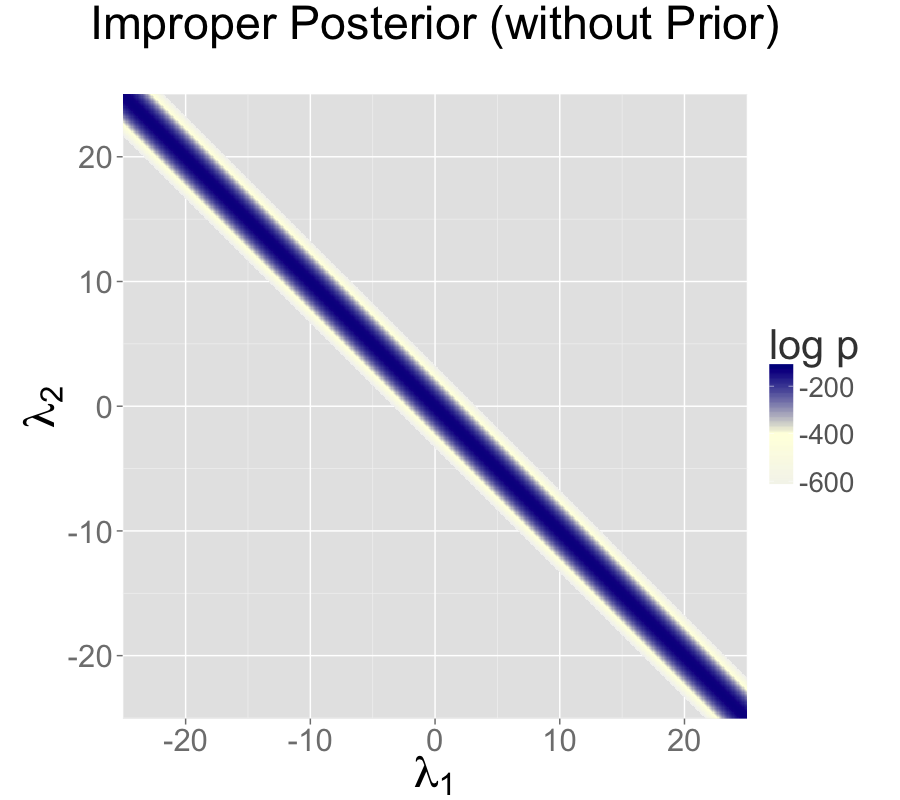
\includegraphics[height=1.45in]{img/non-identified.png}%
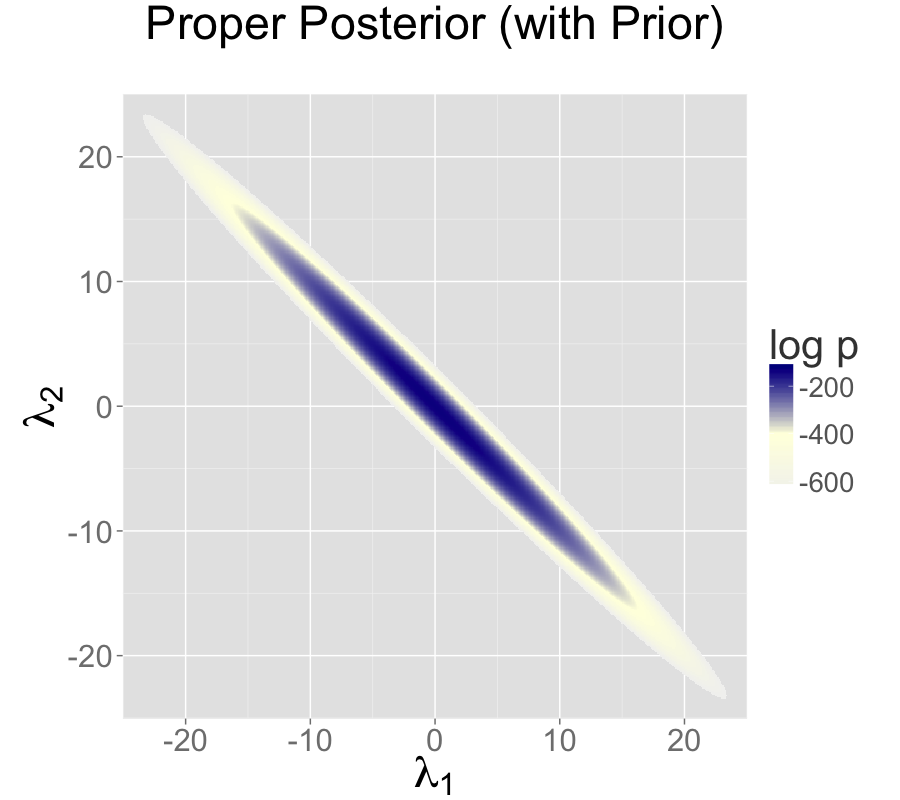
\includegraphics[height=1.45in]{img/non-identified-plus-prior.png}%
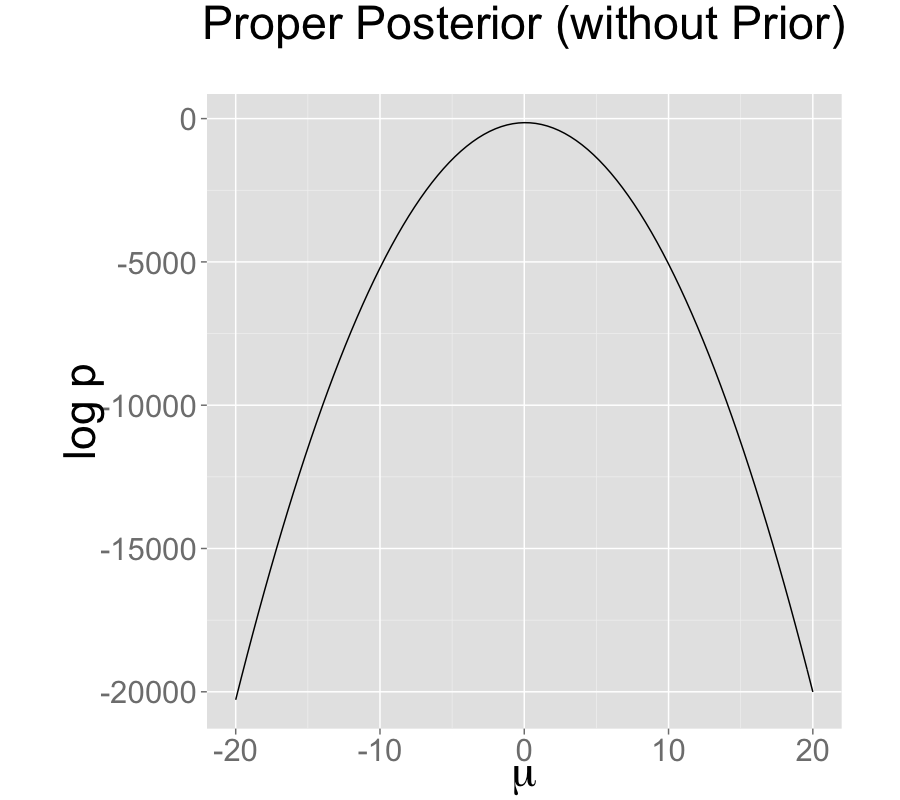
\includegraphics[height=1.45in]{img/one-param-identified.png}
\vspace*{-.1in}
\caption{\small\it Posteriors for two intercept parameterization
  without prior, two intercept parameterization with unit normal
  prior, and one intercept reparameterization without prior.  For all
  three cases, the posterior is plotted for 100 data points drawn from
  a unit normal. Left) The two intercept parameterization leads to an
  improper prior with a ridge extending infinitely to the northwest
  and southeast.  Middle) Adding a unit normal prior for the
  intercepts results in a proper posterior.  Right) The single
  intercept parameterization with no prior also has a proper posterior.}%
\label{non-identifiable-density.figure}
\end{figure}
%
The addition of a prior to the two intercepts model is shown in the
middle plot in \reffigure{non-identifiable-density}.  The plot on
the right of \reffigure{non-identifiable-density} shows the result of
reparameterizing to a single intercept.

An alternative strategy for identifying a $K$-simplex parameterization
$\theta = \mbox{softmax}(\alpha)$ in terms of an unconstrained
$K$-vector $\alpha$ is to place a prior on the components of $\alpha$
with a fixed location (that is, specifically avoid hierarchical priors
with varying location).  Unlike the approaching of pinning $\alpha_K =
0$, the prior-based approach models the $K$ outcomes symmetrically
rather than modeling $K-1$ outcomes relative to the $K$-th.  The
pinned parameterization, on the other hand, is usually more efficient
statistically because it does not have the extra degree of (prior
constrained) wiggle room.


\subsubsection{Vague, Strongly Informative, and Weakly Informative Priors}

Care must be used when adding a prior to resolve invariances.  If the
prior is taken to be too broad (i.e., too vague), the resolution is in
theory only, and samplers will still struggle.

Ideally, a realistic prior will be formulated based on substantive
knowledge of the problem being modeled.  Such a prior can be chosen to
have the appropriate strength based on prior knowledge.  A strongly
informative prior makes sense if there is strong prior information.

When there is not strong prior information, a weakly informative prior
strikes the proper balance between controlling computational inference
without dominating the data in the posterior.  In most problems, the
modeler will have at least some notion of the expected scale of the
estimates and be able to choose a prior for identification purposes
that does not dominate the data, but provides sufficient computational
control on the posterior.

Priors can also be used in the same way to control the additive
invariance of the IRT model.  A typical approach is to place a strong
prior on student ability parameters $\alpha$ to control scale simply
to control the additive invariance of the basic IRT model and the
multiplicative invariance of the model extended with a item
discrimination parameters; such a prior does not add any prior
knowledge to the problem.  Then a prior on item difficulty can be
chosen that is either informative or weakly informative based on prior
knowledge of the problem.


\section{Label Switching in Mixture Models}\label{label-switching-problematic.section}

Where collinearity in regression models can lead to infinitely many
posterior maxima, swapping components in a mixture model leads to
finitely many posterior maxima.

\subsection{Mixture Models}

Consider a normal mixture model with two location parameters $\mu_1$
and $\mu_2$, a shared scale $\sigma > 0$, a mixture ratio $\theta \in
[0,1]$, and likelihood
\[
p(y|\theta,\mu_1,\mu_2,\sigma)
= \prod_{n=1}^N \big( \theta \, \distro{Normal}(y_n|\mu_1,\sigma)
                       + (1 - \theta) \, \distro{Normal}(y_n|\mu_2,\sigma) \big).
\]
The issue here is exchangeability of the mixture components, because
\[
p(\theta,\mu_1,\mu_2,\sigma|y) = p((1-\theta),\mu_2,\mu_1,\sigma|y).
\]
The problem is exacerbated as the number of mixture components $K$
grows, as in clustering models, leading to $K!$ identical posterior
maxima.

\subsection{Convergence Monitoring and Effective Sample Size}

The analysis of posterior convergence and effective sample size is
also difficult for mixture models.  For example, the $\hat{R}$
convergence statistic reported by Stan and the computation of
effective sample size are both compromised by label switching.  The
problem is that the posterior mean, a key ingredient in these
computations, is affected by label switching, resulting in a posterior
mean for $\mu_1$ that is equal to that of $\mu_2$, and a posterior
mean for $\theta$ that is always 1/2, no matter what the data is.

\subsection{Some Inferences are Invariant}

In some sense, the index (or label) of a mixture component is
irrelevant.  Posterior predictive inferences can still be carried out
without identifying mixture components.  For example, the log
probability of a new observation does not depend on the identities of
the mixture components.  The only sound Bayesian inferences in such
models are those that are invariant to label switching.  Posterior
means for the parameters are meaningless because they are not
invariant to label switching; for example, the posterior mean for
$\theta$ in the two component mixture model will always be 1/2.

\subsection{Highly Multimodal Posteriors}

Theoretically, this should not present a problem for inference because
all of the integrals involved in posterior predictive inference will
be well behaved. The problem in practice is computation.

Being able to carry out such invariant inferences in practice is an
altogether different matter.  It is almost always intractable to find
even a single posterior mode, much less balance the exploration of the
neighborhoods of multiple local maxima according to the probability
masses. In Gibbs sampling, it is unlikely for $\mu_1$
to move to a new mode when sampled conditioned on the current values
of $\mu_2$ and $\theta$. For HMC and NUTS, the problem is that the
sampler gets stuck in one of the two ``bowls'' around the modes and
cannot gather enough energy from random momentum assignment to move
from one mode to another.

Even with a proper posterior, all known sampling and inference
techniques are notoriously ineffective when the number of modes grows
super-exponentially as it does for mixture models with increasing
numbers of components.

\subsection{Hacks as Fixes}

Several hacks (i.e., ``tricks'') have been suggested and employed to
deal with the problems posed by label switching in practice.

\subsubsection{Parameter Ordering Constraints}

One common strategy is to impose a constraint on the parameters that
identifies the components.  For instance, we might consider
constraining $\mu_1 < \mu_2$ in the two-component normal mixture model
discussed above.  A problem that can arise from such an approach is
when there is substantial probability mass for the opposite ordering
$\mu_1 > \mu_2$.  In these cases, the posteriors are affected by
the constraint and true posterior uncertainty in $\mu_1$ and $\mu_2$
is not captured by the model with the constraint.  In addition,
standard approaches to posterior inference for event probabilities is
compromised.  For instance, attempting to use $M$ posterior samples to
estimate $\mbox{Pr}[\mu_1 > \mu_2]$, will fail, because the estimator
\[
\mbox{Pr}[\mu_1 > \mu_2]
\approx
\sum_{m=1}^M \mbox{I}(\mu_1^{(m)} > \mu_2^{(m)})
\]
will result in an estimate of 0 because the posterior respects the
constraint in the model.

\subsubsection{Initialization around a Single Mode}

Another common approach is to run a single chain or to initialize the
parameters near realistic values.%
%
\footnote{Tempering methods may be viewed as automated ways to carry
  out such a search for modes, though most MCMC tempering methods
  continue to search for modes on an ongoing basis; see
  \citep{SwendsenWang:1986, Neal:1996b}.}
%
This can work better than the hard constraint approach if reasonable
initial values can be found and the labels do not switch within a
Markov chain.  The result is that all chains are glued to a
neighborhood of a particular mode in the posterior.

\section{Component Collapsing in Mixture Models}

It is possible for two mixture components in a mixture model to
collapse to the same values during sampling or optimization.  For
example, a mixture of $K$ normals might devolve to have $\mu_i =
\mu_j$ and $\sigma_i = \sigma_j$ for $i \neq j$.

This will typically happen early in sampling due to initialization in
MCMC or optimization or arise from random movement during MCMC.  Once
the parameters match for a given draw $(m)$, it can become hard to
escape because there can be a trough of low-density mass between the
current parameter values and the ones without collapsed components.

It may help to use a smaller step size during warmup, a stronger prior
on each mixture component's membership responsibility.  A more extreme
measure is to include additional mixture components to deal with the
possibility that some of them may collapse.

In general, it is very difficult to recover exactly the right $K$
mixture components in a mixture model as $K$ increases beyond one
(yes, even a two-component mixture can have this problem).


\section{Posteriors with Unbounded Densities}

In some cases, the posterior density grows without bounds as
parameters approach certain poles or boundaries.  In such, there
are no posterior modes and numerical stability issues can arise as
sampled parameters approach constraint boundaries.

\subsection{Mixture Models with Varying Scales}

One such example is a binary mixture model with scales varying by
component, $\sigma_1$ and $\sigma_2$ for locations $\mu_1$ and
$\mu_2$. In this situation, the density grows without bound as
$\sigma_1 \rightarrow 0$ and $\mu_1 \rightarrow y_n$ for some $n$;
that is, one of the mixture components concentrates all of its mass
around a single data item $y_n$.

\subsection{Beta-Binomial Models with Skewed Data and Weak Priors}

Another example of unbounded densities arises with a posterior such as
$\distro{Beta}(\phi|0.5,0.5)$, which can arise if very ``weak'' beta
priors are used for groups that have no data. This density is
unbounded as $\phi \rightarrow 0$ and $\phi \rightarrow 1$. Similarly,
a Bernoulli likelihood model coupled with a ``weak'' beta prior, leads
to a posterior
%
\begin{eqnarray*}
p(\phi|y)
& \propto & \textstyle
\distro{Beta}(\phi|0.5,0.5) \times \prod_{n=1}^N \distro{Bernoulli}(y_n|\phi)
\\[4pt]
& = &\textstyle
\distro{Beta}(\phi \, | \, 0.5 + \sum_{n=1}^N y_n, \ \ 0.5 + N - \sum_{n=1}^N y_n).
\end{eqnarray*}
%
If $N = 9$ and each $y_n = 1$, the posterior is
$\distro{Beta}(\phi|9.5,0,5)$.  This posterior is unbounded as $\phi
\rightarrow 1$.  Nevertheless, the posterior is proper, and although
there is no posterior mode, the posterior mean is well-defined with a
value of exactly 0.95.

\subsubsection{Constrained vs.\ Unconstrained Scales}

Stan does not sample directly on the constrained $(0,1)$ space for
this problem, so it doesn't directly deal with unconstrained density
values.  Rather, the probability values $\phi$ are logit-transformed
to $(-\infty,\infty)$.  The boundaries at 0 and 1 are pushed out to
$-\infty$ and $\infty$ respectively.  The Jacobian adjustment that
Stan automatically applies ensures the unconstrained density is
proper.  The adjustment for the particular case of $(0,1)$ is $\log
\mbox{logit}^{-1}(\phi) + \log \mbox{logit}(1 - \phi)$; see
\refsection{logit-transform-jacobian} for the derivation.

There are two problems that still arise, though.  The first is that if
the posterior mass for $\phi$ is near one of the boundaries, the
logit-transformed parameter will have to sweep out very long paths and
thus can dominate the U-turn condition imposed by the no-U-turn
sampler (NUTS).  The second issue is that the inverse transform from
the unconstrained space to the constrained space can underflow to 0 or
overflow to 1, even when the unconstrained parameter is not infinite.
Similar problems arise for the expectation terms in logistic
regression, which is why the logit-scale parameterizations of the
Bernoulli and binomial distributions are more stable.



\section{Posteriors with Unbounded Parameters}

In some cases, the posterior density will not grow without bound, but
parameters will grow without bound with gradually increasing density
values.  Like the models discussed in the previous section that have
densities that grow without bound, such models also have no posterior
modes.


\subsection{Separability in Logistic Regression}

Consider a logistic regression model with $N$ observed outcomes $y_n
\in \{ 0, 1 \}$, an $N \times K$ matrix $x$ of predictors, a
$K$-dimensional coefficient vector $\beta$, and sampling distribution
\[
y_n \sim \distro{Bernoulli}(\mbox{logit}^{-1}(x_n \beta)).
\]
Now suppose that column $k$ of the predictor matrix is such that
$x_{n,k} > 0$ if and only if $y_n = 1$, a condition known as
``separability.''  In this case, predictive accuracy on the observed data
continue to improve as $\beta_k \rightarrow \infty$, because for cases
with $y_n = 1$, $x_n \beta \rightarrow \infty$ and hence
$\mbox{logit}^{-1}(x_n \beta) \rightarrow 1$.

With separability, there is no maximum to the likelihood and hence no
maximum likelihood estimate.  From the Bayesian perspective, the
posterior is improper and therefore the marginal posterior mean for
$\beta_k$ is also not defined.  The usual solution to this problem in
Bayesian models is to include a proper prior for $\beta$, which
ensures a proper posterior.


\section{Uniform Posteriors}

Suppose your model includes a parameter $\psi$ that is defined on
$[0,1]$ and is given a flat prior $\distro{Uniform}(\psi|0,1)$. Now if
the data don't tell us anything about $\psi$, the posterior is also
$\distro{Uniform}(\psi|0,1)$.

Although there is no maximum likelihood estimate for $\psi$, the
posterior is uniform over a closed interval and hence proper.  In the
case of a uniform posterior on $[0,1]$, the posterior mean for $\psi$
is well-defined with value $1/2$.  Although there is no posterior
mode, posterior predictive inference may nevertheless do the right
thing by simply integrating (i.e., averaging) over the predictions for
$\psi$ at all points in $[0,1]$.


\section{Sampling Difficulties with Problematic Priors}

With an improper posterior, it is theoretically impossible to properly
explore the posterior. However, Gibbs sampling as performed by BUGS
and JAGS, although still unable to properly sample from such an
improper posterior, behaves quite differently in practice than the
Hamiltonian Monte Carlo sampling performed by Stan when faced with an
example such as the two intercept model discussed in
\refsection{collinearity} and illustrated in
\reffigure{non-identifiable-density}.

\subsection{Gibbs Sampling}

Gibbs sampling, as performed by BUGS and JAGS, may appear to be
efficient and well behaved for this unidentified model, but as
discussed in the previous subsection, will not actually explore the
posterior properly.

Consider what happens with initial values $\lambda_1^{(0)}, \lambda_2^{(0)}$.
Gibbs sampling proceeds in iteration $m$ by drawing
%
\begin{eqnarray*}
\lambda_1^{(m)}
& \sim & p(\lambda_1 \, | \, \lambda_2^{(m-1)}, \, \sigma^{(m-1)}, \, y)
\\[6pt]
\lambda_2^{(m)}
& \sim & p(\lambda_2 \, | \, \lambda_1^{(m)}, \, \sigma^{(m-1)}, \, y)
\\[6pt]
\sigma^{(m)}
& \sim & p(\sigma \, | \, \lambda_1^{(m)}, \, \lambda_2^{(m)}, \, y).
\end{eqnarray*}
%
Now consider the draw for $\lambda_1$ (the draw for $\lambda_2$ is
symmetric), which is conjugate in this model and thus can be done very
efficiently.  In this model, the range from which the next $\lambda_1$
can be drawn is highly constrained by the current values of
$\lambda_2$ and $\sigma$.  Gibbs will run very quickly and provide
seemingly reasonable inferences for $\lambda_1 + \lambda_2$.  But it
will not explore the full range of the posterior; it will merely take
a slow random walk from the initial values.  This random walk behavior
is typical of Gibbs sampling when posteriors are highly correlated and
the primary reason to prefer Hamiltonian Monte Carlo to Gibbs sampling
for models with parameters correlated in the posterior.

\subsection{Hamiltonian Monte Carlo Sampling}

Hamiltonian Monte Carlo (HMC), as performed by Stan, is much more
efficient at exploring posteriors in models where parameters are
correlated in the posterior.  In this particular example, the
Hamiltonian dynamics (i.e., the motion of a fictitious particle given
random momentum in the field defined by the negative log posterior) is
going to run up and down along the valley defined by the potential
energy (ridges in log posteriors correspond to valleys in potential
energy).  In practice, even with a random momentum for $\lambda_1$ and
$\lambda_2$, the gradient of the log posterior is going to adjust for
the correlation and the simulation will run $\lambda_1$ and
$\lambda_2$ in opposite directions along the valley corresponding to
the ridge in the posterior log density (see
\reffigure{non-identifiable-density}.

\subsection{No-U-Turn Sampling}

Stan's default no-U-turn sampler (NUTS), is even more efficient at
exploring the posterior (see
\citep{Hoffman-Gelman:2011,Hoffman-Gelman:2014}).  NUTS simulates the
motion of the fictitious particle representing the parameter values
until it makes a U-turn, it will be defeated in most cases, as it will
just move down the potential energy valley indefinitely without making
a U-turn. What happens in practice is that the maximum number of
leapfrog steps in the simulation will be hit in many of the
iterations, causing a very large number of log probability and
gradient evaluations (1000 if the max tree depth is set to 10, as in
the default). Thus sampling will appear to be very slow.  This is
indicative of an improper posterior, not a bug in the NUTS algorithm
or its implementation.  It is simply not possible to sample from an
improper posterior!  Thus the behavior of HMC in general and NUTS
in particular should be reassuring in that it will clearly fail in
cases of improper posteriors, resulting in a clean diagnostic of
sweeping out very large paths in the posterior.

\begin{figure}
%
\normalsize {\it Two Scale Parameters, Improper Prior}
%
\footnotesize
\begin{Verbatim}
Inference for Stan model: improper_stan
Warmup took (2.7, 2.6, 2.9, 2.9) seconds, 11 seconds total
Sampling took (3.4, 3.7, 3.6, 3.4) seconds, 14 seconds total

                  Mean     MCSE   StdDev        5%       95%  N_Eff  N_Eff/s  R_hat
lp__          -5.3e+01  7.0e-02  8.5e-01  -5.5e+01  -5.3e+01    150       11    1.0
n_leapfrog__   1.4e+03  1.7e+01  9.2e+02   3.0e+00   2.0e+03   2987      212    1.0
lambda1        1.3e+03  1.9e+03  2.7e+03  -2.3e+03   6.0e+03    2.1     0.15    5.2
lambda2       -1.3e+03  1.9e+03  2.7e+03  -6.0e+03   2.3e+03    2.1     0.15    5.2
sigma          1.0e+00  8.5e-03  6.2e-02   9.5e-01   1.2e+00     54      3.9    1.1
mu             1.6e-01  1.9e-03  1.0e-01  -8.3e-03   3.3e-01   2966      211    1.0
\end{Verbatim}
%
\vspace*{12pt}
%
\normalsize
{\it Two Scale Parameters, Weak Prior}
%
\footnotesize
\begin{Verbatim}
Warmup took (0.40, 0.44, 0.40, 0.36) seconds, 1.6 seconds total
Sampling took (0.47, 0.40, 0.47, 0.39) seconds, 1.7 seconds total

                 Mean     MCSE   StdDev        5%    95%  N_Eff  N_Eff/s  R_hat
lp__              -54  4.9e-02  1.3e+00  -5.7e+01    -53    728      421    1.0
n_leapfrog__      157  2.8e+00  1.5e+02   3.0e+00    511   3085     1784    1.0
lambda1          0.31  2.8e-01  7.1e+00  -1.2e+01     12    638      369    1.0
lambda2         -0.14  2.8e-01  7.1e+00  -1.2e+01     12    638      369    1.0
sigma             1.0  2.6e-03  8.0e-02   9.2e-01    1.2    939      543    1.0
mu               0.16  1.8e-03  1.0e-01  -8.1e-03   0.33   3289     1902    1.0
\end{Verbatim}
%
\vspace*{12pt}
%
\normalsize {\it One Scale Parameter, Improper Prior}
%
\footnotesize
\begin{Verbatim}
Warmup took (0.011, 0.012, 0.011, 0.011) seconds, 0.044 seconds total
Sampling took (0.017, 0.020, 0.020, 0.019) seconds, 0.077 seconds total

                Mean     MCSE  StdDev        5%   50%   95%  N_Eff  N_Eff/s  R_hat
lp__             -54  2.5e-02    0.91  -5.5e+01   -53   -53   1318    17198    1.0
n_leapfrog__     3.2  2.7e-01     1.7   1.0e+00   3.0   7.0     39      507    1.0
mu              0.17  2.1e-03    0.10  -3.8e-03  0.17  0.33   2408    31417    1.0
sigma            1.0  1.6e-03   0.071   9.3e-01   1.0   1.2   2094    27321    1.0
\end{Verbatim}
%
\caption{\small\it Results of Stan runs with default parameters fit to
  $N=100$ data points generated from $y_n \sim \distro{Normal}(0,1)$.
  %
  On the top is the non-identified model with improper uniform priors
  and likelihood $y_n \sim \distro{Normal}(\lambda_1 + \lambda_2,
  \sigma)$.
  %
  In the middle is the same likelihood as the middle plus priors
  $\lambda_k \sim \distro{Normal}(0,10)$.
  %
  On the bottom is an identified model with an improper prior, with
  likelihood  $y_n \sim \distro{Normal}(\mu,\sigma)$.  All models
  estimate $\mu$ at roughly 0.16 with very little Monte Carlo standard
  error, but a high posterior standard deviation of 0.1;  the true
  value $\mu=0$ is within the 90\% posterior intervals in all three models.
  %
}%
\label{non-identified-stan-fits.figure}
\end{figure}
%

\subsection{Examples: Fits in Stan}

To illustrate the issues with sampling from non-identified and only
weakly identified models, we fit three models with increasing degrees
of identification of their parameters.  The posteriors for these
models is illustrated in \reffigure{non-identifiable-density}.  The
first model is the unidentified model with two location parameters and
no priors discussed in \refsection{collinearity}.
%
\begin{stancode}
data {
  int N;
  real y[N];
}
parameters {
  real lambda1;
  real lambda2;
  real<lower=0> sigma;
}
transformed parameters {
  real mu;
  mu = lambda1 + lambda2;
}
model {
  y ~ normal(mu, sigma);
}
\end{stancode}
%
The second adds priors to the model block for \code{lambda1} and
\code{lambda2} to the previous model.
%
\begin{stancode}
  lambda1 ~ normal(0, 10);
  lambda2 ~ normal(0, 10);
\end{stancode}
%
The third involves a single location parameter, but no priors.
%
\begin{stancode}
data {
  int N;
  real y[N];
}
parameters {
  real mu;
  real<lower=0> sigma;
}
model {
  y ~ normal(mu, sigma);
}
\end{stancode}
%
All three of the example models were fit in Stan 2.1.0 with default
parameters (1000 warmup iterations, 1000 sampling iterations, NUTS
sampler with max tree depth of 10). The results are shown in
\reffigure{non-identified-stan-fits}. The key statistics from these
outputs are the following.
%
\begin{itemize}
\item As indicated by \code{R\_hat} column, all parameters have
  converged other than $\lambda_1$ and $\lambda_2$ in the
  non-identified model.
\item
  The average number of leapfrog steps is roughly 3 in
  the identified model, 150 in the model identified by a weak prior, and
  1400 in the non-identified model.
\item
  The number of effective samples per
  second for $\mu$ is roughly 31,000 in the identified model, 1900 in the model
  identified with weakly informative priors, and 200 in the
  non-identified model; the results are similar for $\sigma$.
\item
  In the non-identified model, the 95\% interval for $\lambda_1$ is
  (-2300,6000), whereas it is only (-12,12) in the model identified with
  weakly informative priors.
\item
  In all three models, the simulated value of $\mu=0$ and $\sigma=1$
  are well within the posterior 90\% intervals.
\end{itemize}
%
The first two points, lack of convergence and hitting the maximum
number of leapfrog steps (equivalently maximum tree depth) are
indicative of improper posteriors.  Thus rather than covering up the
problem with poor sampling as may be done with Gibbs samplers,
Hamiltonian Monte Carlo tries to explore the posterior and its failure
is a clear indication that something is amiss in the model.


\chapter{Matrices, Vectors, and Arrays}

\noindent
This chapter provides pointers as to how to choose among the various
matrix, vector, and array data structures provided by Stan.

\section{Basic Motivation}

Stan provides two basic scalar types, \code{int} and \code{real}, and
three basic linear algebra types, \code{vector}, \code{row\_vector},
and \code{matrix}.  Then Stan allows arrays to be of any dimension and
contain any type of element (though that type must be declared and
must be the same for all elements).

This leaves us in the awkward situation of having three
one-dimensional containers, as exemplified by the following
declarations.
%
\begin{stancode}
real a[N];
vector[N] a;
row_vector[N] a;
\end{stancode}
%
These distinctions matter.  Matrix types, like vector and row vector,
are required for linear algebra operations.  There is no automatic
promotion of arrays to vectors because the target, row vector or
column vector, is ambiguous.  Similarly, row vectors are separated
from column vectors because multiplying a row vector by a column
vector produces a scalar, whereas multiplying in the opposite order
produces a matrix.

The following code fragment shows all four ways to declare a
two-dimensional container of size $M \times N$.
%
\begin{stancode}
real b[M, N];          // b[m] : real[]     (efficient)
vector[N] b[M];        // b[m] : vector     (efficient)
row_vector[N] b[M];    // b[m] : row_vector (efficient)
matrix[M, N] b;        // b[m] : row_vector (inefficient)
\end{stancode}
%
The main differences among these choices involve efficiency for
various purposes and the type of \code{b[m]}, which is shown in
comments to the right of the declarations.  Thus the only way to
efficiently iterate over row vectors is to use the third declaration,
but if you need linear algebra on matrices, but the only way to use
matrix operations is to use the fourth declaration.

The inefficiencies due to any manual reshaping of containers is
usually slight compared to what else is going on in a Stan program
(typically a lot of gradient calculations).


\section{Fixed Sizes and Indexing out of Bounds}

Stan's matrices, vectors, and array variables are sized when they are
declared and may not be dynamically resized.  Function arguments do
not have sizes, but these sizes are fixed when the function is called
and the container is instantiated.  Also, declarations may be inside
loops and thus may change over the course of running a program, but
each time a declaration is visited, it declares a fixed size object.

When an index is provided that is out of bounds, Stan throws a
rejection error and computation on the current log density and
gradient evaluation is halted and the algorithm is left to clean up
the error.  All of Stan's containers check the sizes of all indexes.



\section{Data Type and Indexing Efficiency}\label{indexingefficiency.section}

The underlying matrix and linear algebra operations are implemented in
terms of data types from the Eigen \Cpp library.  By having vectors
and matrices as basic types, no conversion is necessary when invoking
matrix operations or calling linear algebra functions.

Arrays, on the other hand, are implemented as instances of the \Cpp \
\code{std::vector} class (not to be confused with Eigen's
\code{Eigen::Vector} class or Stan vectors).  By implementing arrays
this way, indexing is very efficient because values can be returned by
reference rather than copied by value.

\subsection{Matrices vs.\ Two-Dimensional Arrays}

In Stan models, there are a few minor efficiency considerations in
deciding between a two-dimensional array and a matrix, which may seem
interchangeable at first glance.

First, matrices use a bit less memory than two-dimensional arrays.
This is because they don't store a sequence of arrays, but just the
data and the two dimensions.

Second, matrices store their data in column-major order.  Furthermore,
all of the data in a matrix is guaranteed to be contiguous in memory.
This is an important consideration for optimized code because bringing
in data from memory to cache is much more expensive than performing
arithmetic operations with contemporary CPUs.  Arrays, on the other
hand, only guarantee that the values of primitive types are contiguous
in memory; otherwise, they hold copies of their values (which are
returned by reference wherever possible).

Third, both data structures are best traversed in the order in which
they are stored.  This also helps with memory locality.  This is
column-major for matrices, so the following order is appropriate.
%
\begin{stancode}
matrix[M, N] a;
//...
for (n in 1:N)
  for (m in 1:M)
    // ... do something with a[m, n] ...
\end{stancode}
%
Arrays, on the other hand, should be traversed in row-major order
(i.e., last index fastest), as in the following example.
%
\begin{stancode}
real a[M, N];
// ...
for (m in 1:M)
  for (n in 1:N)
    // ... do something with a[m, n] ...
\end{stancode}
%
The first use of \code{a[m,~n]} should bring \code{a[m]} into memory.
Overall, traversing matrices is more efficient than traversing arrays.

This is true even for arrays of matrices.  For example, the ideal
order in which to traverse a two-dimensional array of matrices is
%
\begin{stancode}
matrix[M, N] b[I, J];
// ...
for (i in 1:I)
  for (j in 1:J)
    for (n in 1:N)
      for (m in 1:M)
        ... do something with b[i, j, m, n] ...
\end{stancode}

If \code{a} is a matrix, the notation \code{a[m]} picks out row
\code{m} of that matrix.  This is a rather inefficient operation for
matrices.  If indexing of vectors is needed, it is much better to
declare an array of vectors.  That is, this
%
\begin{stancode}
row_vector[N] b[M];
// ...
for (m in 1:M)
   ... do something with row vector b[m] ...
\end{stancode}
%
is much more efficient than the pure matrix version
%
\begin{stancode}
matrix b[M, N];
// ...
for (m in 1:M)
   // ... do something with row vector b[m] ...
\end{stancode}
%
Similarly, indexing an array of column vectors is more efficient than
using the \code{col} function to pick out a column of a matrix.

In contrast, whatever can be done as pure matrix algebra will be the
fastest.  So if I want to create a row of predictor-coefficient
dot-products, it's more efficient to do this
%
\begin{stancode}
matrix[N, k] x;    // predictors (aka covariates)
// ...
vector[K] beta;   // coeffs
// ...
vector[N] y_hat;  // linear prediction
// ...
y_hat = x * beta;
\end{stancode}
%
than it is to do this
%
\begin{stancode}
row_vector[K] x[N];    // predictors (aka covariates)
// ...
vector[K] beta;   // coeffs
...
vector[N] y_hat;  // linear prediction
...
for (n in 1:N)
  y_hat[n] = x[n] * beta;
\end{stancode}

\subsection{(Row) Vectors vs. One-Dimensional Arrays}

For use purely as a container, there is really nothing to decide among
vectors, row vectors and one-dimensional arrays.  The
\code{Eigen::Vector} template specialization and the
\code{std::vector} template class are implemented very similarly as
containers of \code{double} values (the type \code{real} in Stan).
Only arrays in Stan are allowed to store integer values.


\section{Memory Locality}

The key to understanding efficiency of matrix and vector
representations is memory locality and reference passing versus
copying.

\subsection{Memory Locality}

CPUs on computers bring in memory in blocks through layers of caches.
Fetching from memory is \emph{much}\ slower than performing arithmetic
operations.  The only way to make container operations fast is to
respect memory locality and access elements that are close together in
memory sequentially in the program.

\subsection{Matrices}

Matrices are stored internally in column-major order.  That is, an $M
\times N$ matrix stores its elements in the order
\[
(1,1), (2, 1), \ldots, (M, 1), (1, 2), \ldots, (M, 2), \ldots, (1, N),
\ldots, (M, N).
\]
%
This means that it's much more efficient to write loops over matrices
column by column, as in the following example.
%
\begin{stancode}
matrix[M, N] a;
...
for (n in 1:N)
  for (m in 1:M)
     ... do something with a[m, n] ...
\end{stancode}

It also follows that pulling a row out of a matrix is not memory
local, as it has to stride over the whole sequence of values.  It also
requires a copy operation into a new data structure as it is not
stored internally as a unit in a matrix.  For sequential access to row
vectors in a matrix, it is much better to use an array of row vectors,
as in the following example.
%
\begin{stancode}
row_vector[N] a[M];
...
for (m in 1:M)
  ... do something with row vector a[m] ...
\end{stancode}
%
Even if what is done involves a function call, the row vector
\code{a[m]} will not have to be copied.

\subsection{Arrays}

Arrays are stored internally following their data structure.  That
means a two dimensional array is stored in row-major order.  Thus it
is efficient to pull out a ``row'' of a two-dimensional array.
%
\begin{stancode}
real a[M, N];
...
for (m in 1:M)
  ... do something with a[m] ...
\end{stancode}

A difference with matrices is that the entries \code{a[m]} in the two
dimensional array are not necessarily adjacent in memory, so there are
no guarantees on iterating over all the elements in a two-dimensional
array will provide memory locality across the ``rows.''

\section{Converting among Matrix, Vector, and Array Types}

There is no automatic conversion among matrices, vectors, and arrays
in Stan.  But there are a wide range of conversion functions to
convert a matrix into a vector, or a multi-dimensional array into a
one-dimensional array, or convert a vector to an array.  See
\refchapter{mixed-operations} for complete details on the available conversion
operators as well as \refchapter{multi-indexing} for some
reshaping operations involving multiple indexing and range indexing.


\section{Aliasing in Stan Containers}

Stan expressions are all evaluated before assignment happens, so there
is no danger of so-called aliasing in array, vector, or matrix
operations.  Contrast the behavior of the assignments to \code{u} and
\code{x}, which start with the same values.

The loop assigning to \code{u} and the compound slicing assigning to \code{x}.

 the following trivial Stan program.

\begin{stancode}
transformed data {
  vector[4] x = [ 1, 2, 3, 4 ]';
  vector[4] u = [ 1, 2, 3, 4 ]';

  for (t in 2:4)
    u[t] = u[t - 1] * 3;

  x[2:4] = x[1:3] * 3;

  print("u = ", u);
  print("x = ", x);
}
\end{stancode}
%
The output it produces is as follows
%
\begin{stancode}
u = [1,3,9,27]
x = [1,3,6,9]
\end{stancode}
%
In the loop version assiging to \code{u}, the values are updated before being used to
define subseqeunt values;  in the sliced expression assigning to
\code{x}, the entire right-hand side is evaluated before assigning to
the left-hand side.

\chapter{Multiple Indexing and Range Indexing}\label{multi-indexing.chapter}

Stan allows multiple indexes to be provided for containers (i.e.,
arrays, vectors, and matrices) in a single position, using either an
array of integer indexes or range bounds.  This allows many models to
be vectorized.  For instance, consider the likelihood for a varying-slope,
varying-intercept hierarchical linear regression, which could be coded
as
%
\begin{stancode}
for (n in 1:N)
  y[n] ~ normal(alpha[ii[n]] + beta[ii[n]] * x[n], sigma);
\end{stancode}
%
With multiple indexing, this can be coded in one line, leading to more
efficient vectorized code.
%
\begin{stancode}
y ~ normal( rows_dot_product(alpha[ii] + beta[ii] , x), sigma);
\end{stancode}
%
This latter version is equivalent in speed to the clunky assignment to
a local variable.
%
\begin{stancode}
{
  vector[N] mu;
  for (n in 1:N)
    mu[n] = alpha[ii[n]] + beta[ii[n]] * x[n];
  y ~ normal(mu, sigma);
}
\end{stancode}

\section{Multiple Indexing}

The following is the simplest concrete example of multiple indexing
with an array of integers;  the ellipses stand for code defining the
variables as indicated in the comments.
%
\begin{stancode}
int c[3];
...             // define: c == (5, 9, 7)
int idxs[4];
...             // define: idxs == (3, 3, 1, 2)
int d[4];
d = c[idxs];   // result: d == (7, 7, 5, 9)
\end{stancode}
%

In general, the multiple indexed expression \code{c[idxs]} is defined
as follows, assuming \code{idxs} is of size \code{K}.
%
\begin{stancode}
c[idxs] = ( c[idxs[1]], c[idxs[2]], ..., c[idxs[K]] )
\end{stancode}
%
Thus \code{c[idxs]} is of the same size as \code{idxs}, which is
\code{K} in this example.

Multiple indexing can also be used with multi-dimensional arrays.  For
example, consider the following.
%
\begin{stancode}
int c[2, 3];
...            // define: c = ((1, 3, 5), ((7, 11, 13))
int idxs[4];
...            // define: idxs = (2, 2, 1, 2)
int d[4, 3]
d = c[idxs];  // result: d = ((7, 11, 13), (7, 11, 13),
               //              (1, 3, 5), (7, 11, 13))
\end{stancode}
%
That is, putting an index in the first position acts exactly the same
way as defined above.  The fact that the values are themselves arrays
makes no difference---the result is still defined by \code{c[idxs][j] ==
  c[idxs[j]]}.

Multiple indexing may also be used in the second position of a
multi-dimensional array.  Continuing the above example, consider a
single index in the first position and a multiple index in the second.
%
\begin{stancode}
int e[4];
e = c[2, idxs];  // result:  c[2] = (7, 11, 13)
                  // result:  e = (11, 11, 7, 11)
\end{stancode}
%
The single index is applied, the one-dimensional result is determined,
then the multiple index is applied to the result.  That is,
\code{c[2,idxs]} evaluates to the same value as \code{c[2][idxs]}.

Multiple indexing can apply to more than one position of a
multi-dimensional array.  For instance, consider the following
%
\begin{stancode}
int c[2, 3];
...                    // define: c = ((1, 3, 5), (7, 11, 13))
int idxs1[3];
...                    // define: idxs1 = (2, 2, 1)
int idxs2[2];
...                    // define: idxs2 = (1, 3)
int d[3, 2];
d = c[idxs1, idxs2];  // result: d = ((7, 13), (7, 13), (1, 5))
\end{stancode}
%
With multiple indexes, we no longer have \code{c[idxs1,~idxs2]} being
the same as \code{c[idxs1][idxs2]}.  Rather, the entry \code{d[i,~j]}
after executing the above is given by
%
\begin{stancode}
d[i, j] == c[idxs1, idxs2][i, j] = c[idxs1[i], idxs2[j]]
\end{stancode}
%
This example illustrates the operation of multiple indexing in the
general case: a multiple index like \code{idxs1} converts an index
\code{i} used on the result (here, \code{c[idxs1, idxs2]}) to index
\code{idxs1[i]} in the variable being indexed (here, \code{c}).  In
contrast, a single index just returns the value at that index, thus
reducing dimensionality by one in the result.

\section{Slicing with Range Indexes}

Slicing returns a contiguous slice of a one-dimensional array, a
contiguous sub-block of a two-dimensional array, and so on.
Semantically, it is just a special form of multiple indexing.

\subsection{Lower and Upper Bound Indexes}

For instance, consider supplying an upper and lower bound for an
index.
%
\begin{stancode}
int c[7];
...
int d[4];
d = c[3:6];  // result: d == (c[3], c[4], c[5], c[6])
\end{stancode}
%
The range index \code{3:6} behaves semantically just like the multiple
index \code{(3, 4, 5, 6)}.  In terms of implementation, the sliced
upper and/or lower bounded indices are faster and use less memory
because they do not explicitly create a multiple index, but rather use
a direct loop.  They are also easier to read, so should be preferred
over multiple indexes where applicable.

\subsection{Lower or Upper Bound Indexes}

It is also possible to supply just a lower bound, or just an upper
bound.  Writing \code{c[3:]} is just shorthand for
\code{c[3:size(c)]}.  Writing \code{c[:5]} is just shorthand for
\code{c[1:5]}.

\subsection{Full Range Indexes}

Finally, it is possible to write a range index that covers the entire
range of an array, either by including just the range symbol
(\code{:}) as the index or leaving the index position empty. In both
cases, \code{c[]} and \code{c[:]} are equal to \code{c[1:size(c)]},
which in turn is just equal to \code{c}.

\section{Multiple Indexing on the Left of Assignments}

Multiple expressions may be used on the left-hand side of an
assignment statement, where they work exactly the same way as on the
right-hand side in terms of picking out entries of a container.
For example, consider the following.
%
\begin{stancode}
int a[3];
int c[2];
int idxs[2];
...             // define: a == (1, 2, 3);  c == (5, 9)
                //         idxs = (3,2)
a[idxs] = c;   // result: a == (1, 9, 5)
\end{stancode}
%
The result above can be worked out by noting that the assignment sets
\code{a[idxs[1]]} (\code{a[3]}) to \code{c[1]} (\code{5}) and
\code{a[idxs[2]]} (\code{a[2]}) to \code{c[2]} (\code{9}).

The same principle applies when there are many multiple indexes, as
in the following example.
%
\begin{stancode}
int a[5, 7];
int c[2, 2];
...
a[2:3, 5:6] = c;  // result: a[2, 5] == c[1, 1];  a[2, 6] == c[1, 2]
                   //         a[3, 5] == c[2, 1];  a[3, 6] == c[2, 2]
\end{stancode}
%
As in the one-dimensional case, the right-hand side is written into
the slice, block, or general chunk picked out by the left-hand side.

Usage on the left-hand side allows the full generality of multiple
indexing, with single indexes reducing dimensionality and multiple
indexes maintaining dimensionality while rearranging, slicing, or
blocking.  For example, it is valid to assign to a segment of a row of
an array as follows.
%
\begin{stancode}
int a[10, 13];
int c[2];
...
a[4, 2:3] = c;  // result:  a[4, 2] == c[1];  a[4, 3] == c[2]
\end{stancode}

\subsection{Assign-by-Value and Aliasing}

Aliasing issues arise when there are references to the same data
structure on the right-hand and left-hand side of an assignment.  For
example, consider the array \code{a} in the following code fragment.
%
\begin{stancode}
int a[3];
...                // define: a == (5, 6, 7)
a[2:3] = a[1:2];
...                // result: a == (5, 5, 6)
\end{stancode}
%
The reason the value of \code{a} after the assignment is $(5,5,6)$
rather than $(5,5,5)$ is that Stan behaves as if the right-hand side
expression is evaluated to a fresh copy.   As another example,
consider the following.
%
\begin{stancode}
int a[3];
int idxs[3];
...            // define idxs = (2, 1, 3)
a[idxs] = a;
\end{stancode}
%
In this case, it is evident why the right-hand side needs to be copied
before the assignment.

It is tempting (but wrong) to think of the assignment \code{a[2:3] =
  a[1:2]} as executing the following assignments.
%
\begin{stancode}
...                // define: a = (5, 6, 7)
a[2] = a[1];      // result: a = (5, 5, 7)
a[3] = a[2];      // result: a = (5, 5, 5)!
\end{stancode}
%
This produces a different result than executing the assignment because
\code{a[2]}'s value changes before it is used.


\section{Multiple Indexes with Vectors and Matrices}

Multiple indexes can be supplied to vectors and matrices as well as
arrays of vectors and matrices.

\subsection{Vectors}

Vectors and row vectors behave exactly the same way as arrays with
multiple indexes.  If \code{v} is a vector, then \code{v[3]} is a
scalar real value, whereas \code{v[2:4]} is a vector of size 3
containing the elements \code{v[2]}, \code{v[3]}, and \code{v[4]}.

The only subtlety with vectors is in inferring the return type when
there are multiple indexes. For example, consider the following
minimal example.
%
\begin{stancode}
vector[5] v[3];
int idxs[7];
...
vector[7] u;
u = v[2, idxs];

real w[7];
w = v[idxs, 2];
\end{stancode}
%
The key is understanding that a single index always reduces
dimensionality, whereas a multiple index never does.  The dimensions
with multiple indexes (and unindexed dimensions) determine the indexed
expression's type.  In the example above, because \code{v} is an array
of vectors, \code{v[2,~idxs]} reduces the array dimension but doesn't
reduce the vector dimension, so the result is a vector.  In contrast,
\code{v[idxs,~2]} does not reduce the array dimension, but does reduce
the vector dimension (to a scalar), so the result type for \code{w} is
an array of reals.  In both cases, the size of the multiple index
(here, 7) determines the size of the result.

\subsection{Matrices}

Matrices are a bit trickier because they have two dimensions, but the
underlying principle of type inference is the same---multiple indexes
leave dimensions in place, whereas single indexes reduce them.  The
following code shows how this works for multiple indexing of matrices.
%
\begin{stancode}
matrix[5,7] m;
...
row_vector[3] rv;
rv = m[4, 3:5];    // result is 1 x 3
...
vector[4] v;
v = m[2:5, 3];     // result is 3 x 1
...
matrix[3, 4] m2;
m2 = m[1:3, 2:5];  // result is 3 x 4
\end{stancode}
%
The key is realizing that any position with a multiple index or
bounded index remains in play in the result, whereas any dimension
with a single index is replaced with 1 in the resulting dimensions.
Then the type of the result can be read off of the resulting
dimensionality as indicated in the comments above.

\subsection{Matrices with One Multiple Index}

If matrices receive a single multiple index, the result is a matrix.
So if \code{m} is a matrix, so is \code{m[2:4]}.  In contrast,
supplying a single index, \code{m[3]}, produces a row vector result.
That is, \code{m[3]} produces the same result as \code{m[3,~]}
or \code{m[3,~1:cols(m)]}.

\subsection{Arrays of Vectors or Matrices}

With arrays of matrices, vectors, and row vectors, the basic access
rules remain exactly the same: single indexes reduce dimensionality
and multiple indexes redirect indexes.  For example, consider the
following example.
%
\begin{stancode}
matrix[3, 4] m[5, 7];
...
matrix[3, 4] a[2];
a = m[1, 2:3];  // knock off first array dimension
a = m[3:4, 5];  // knock off second array dimension
\end{stancode}
%
In both assignments, the multiple index knocks off an array dimension,
but it's different in both cases.  In the first case, \code{a[i] ==
  m[1, i + 1]}, whereas in the second case, \code{a[i] == m[i + 2,
  5]}.

Continuing the previous example, consider the following.
%
\begin{stancode}
...
vector[2] b;
b = a[1, 3, 2:3, 2];
\end{stancode}
%
Here, the two array dimensions are reduced as is the column dimension
of the matrix, leaving only a row dimension index, hence the result is
a vector.  In this case, \code{b[j] == a[1, 3, 1 + j, 2]}.

This last example illustrates an important point: if there is a
lower-bounded index, such as \code{2:3}, with lower bound 2, then the
lower bound minus one is added to the index, as seen in the \code{1 +
  j} expression above.

Continuing further, consider continuing with the following.
%
\begin{stancode}
...
row_vector[3] c[2];
c = a[4:5, 3, 1, 2: ];
\end{stancode}
%
Here, the first array dimension is reduced, leaving a single array
dimension, and the row index of the matrix is reduced, leaving a row
vector.  For indexing, the values are given by
\code{c[i, j] == a[i + 3, 3, 1, j + 1]}


\section{Matrices with Parameters and Constants}

Suppose you have a $3 x 3$ matrix and know that two entries are zero but the
others are parameters.  Such a situation arises in missing data
situations and in problems with fixed structural parameters.

Suppose a $3 \times 3$ matrix is known to be zero at indexes $[1,2]$
and $[1,3]$.  The indexes for parameters are included in a ``melted''
data-frame or database format.

\begin{stancode}
transformed data {
  int<lower=1, upper=3> idxs[7, 2]
    = { {1, 1},
        {2, 1}, {2, 2}, {2, 3},
        {3, 1}, {3, 2}, {3, 3} };
  ...
\end{stancode}
%
The seven remaining parameters are declared as a vector.
%
\begin{stancode}
parameters {
  vector[7] A_raw;
  ...
\end{stancode}
%
Then the full matrix \code{A} is constructed in the model block as a
local variable.
%
\begin{stancode}
model {
  matrix[3, 3] A;
  for (i in 1:7)
    A[idxs[i, 1], idxs[i, 2]] = A_raw[i];
  A[1, 2] = 0;
  A[1, 3] = 0;
  ...
\end{stancode}
%
This may seem like overkill in this setting, but in more general
settings, the matrix size, vector size, and the \code{idxs} array will
be too large to code directly.  Similar techniques can be used to
build up matrices with ad-hoc constraints, such as a handful of
entries known to be positive.



\chapter{Optimizing Stan Code for Efficiency}\label{optimization.chapter}
\noindent
This chapter provides a grab bag of techniques for optimizing Stan
code, including vectorization, sufficient statistics, and conjugacy.
At a coarse level, efficiency involves both the amount of time
required for a computation and the amount of memory required.  For
practical applied statistical modeling, we are mainly concerned with
reducing wall time (how long a program takes as measured by a clock on
the wall) and keeping memory requirements within available bounds.

\section{What is Efficiency?}

The standard algorithm analyses in computer science measure efficiency
asymptotically as a function of problem size (such as data, number of
parameters, etc.) and typically do not consider constant additive
factors like startup times or multiplicative factors like speed of
operations.  In practice, the constant factors are important; if run
time can be cut in half or more, that's a huge gain. This chapter
focuses on both the constant factors involved in efficiency (such as
using built-in matrix operations as opposed to naive loops) and on
asymptotic efficiency factors (such as using linear algorithms instead
of quadratic algorithms in loops).


\section{Efficiency for Probabilistic Models and Algorithms}

Stan programs express models which are intrinsically statistical in
nature.  The algorithms applied to these models may or may not
themselves be probabilistic.  For example, given an initial value for
parameters (which may itself be given deterministically or generated
randomly), Stan's optimization algorithm (L-BFGS) for penalized
maximum likelihood estimation is purely deterministic.  Stan's
sampling algorithms are based on Markov chain Monte Carlo algorithms,
which are probabilistic by nature at every step.  Stan's variational
inference algorithm (ADVI) is probabilistic despite being an
optimization algorithm; the randomization lies in a nested Monte Carlo
calculation for an expected gradient.

With probabilistic algorithms, there will be variation in run times
(and maybe memory usage) based on the randomization involved.  For
example, by starting too far out in the tail, iterative algorithms
underneath the hood, such as the solvers for ordinary differential
equations, may take different numbers of steps.  Ideally this
variation will be limited;  when there is a lot of variation it can be
a sign that there is a problem with the model's parameterization in
a Stan program or with initialization.

A well-behaved Stan program will have low variance between runs with
different random initializations and differently seeded random number
generators.  But sometimes an algorithm can get stuck in one part of
the posterior, typically due to high curvature.  Such sticking almost
always indicates the need to reparameterize the model.  Just throwing
away Markov chains with apparently poor behavior (slow, or stuck) can
lead to bias in posterior estimates.  This problem with getting stuck
can often be overcome by lowering the initial step size to avoid
getting stuck during adaptation and increasing the target acceptance
rate in order to target a lower step size.  This is because smaller
step sizes allow Stan's gradient-based algorithms to better follow the
curvature in the density or penalized maximum likelihood being fit.

\section{Statistical vs.\  Computational Efficiency}

There is a difference between pure computational efficiency and
statistical efficiency for Stan programs fit with sampling-based
algorithms.  Computational efficiency measures the amount of time or
memory required for a given step in a calculation, such as an
evaluation of a log posterior or penalized likelihood.

Statistical efficiency typically involves requiring fewer steps in
algorithms by making the statistical formulation of a model better
behaved.  The typical way to do this is by applying a change of
variables (i.e., reparameterization) so that sampling algorithms mix
better or optimization algorithms require less adaptation.

\section{Model Conditioning and Curvature}

Because Stan's algorithms (other than Riemannian Hamiltonian Monte
Carlo) rely on step-based gradient-based approximations of the density
(or penalized maximum likelihood) being fitted, posterior curvature
not captured by this first-order approximation plays a central role in
determining the statistical efficiency of Stan's algorithms.

A second-order approximation to curvature is provided by the
Hessian, the matrix of second derivatives of the log density $\log
p(\theta)$ with respect to the parameter vector $\theta$, defined
as
\[
H(\theta) = \nabla \, \nabla \, \log p(\theta | y),
\]
so that
\[
H_{i, j}(\theta) = \frac{\partial^2 \log p(\theta | y)}
                {\partial \theta_i \ \partial \theta_j}.
\]
For pure penalized maximum likelihood problems, the posterior log
density $\log p(\theta | y)$ is replaced by the penalized likelihood
function $\mathcal{L}(\theta) = \log p(y | \theta) - \lambda(\theta)$.

\subsection{Condition Number and Adaptation}

A good gauge of how difficult a problem the curvature presents is
given by the condition number of the Hessian matrix $H$, which is the
ratio of the largest to the smallest eigenvalue of $H$ (assuming the
Hessian is positive definite).  This essentially measures the
difference between the flattest direction of movement and the most
curved.  Typically, the step size of a gradient-based algorithm is
bounded by the most sharply curved direction.  With better conditioned
log densities or penalized likelihood functions, it is easier for
Stan's adaptation, especially the diagonal adaptations that are used
as defaults.

\subsection{Unit Scales without Correlation}

Ideally, all parameters should be programmed so that they have unit
scale and so that posterior correlation is reduced; together, these
properties mean that there is no rotation or scaling required for
optimal performance of Stan's algorithms.  For Hamiltonian Monte
Carlo, this implies a unit mass matrix, which requires no adaptation
as it is where the algorithm initializes.  Riemannian Hamiltonian
Monte Carlo performs this conditioning on the fly at every step, but
such conditioning is very expensive computationally.

\subsection{Varying Curvature}

In all but very simple models (such as multivariate normals), the
Hessian will vary as $\theta$ varies.  As an example, see the
illustration of Neal's funnel example in \reffigure{funnel}.  The more
the curvature varies, the harder it is for all of the algorithms with
fixed adaptation parameters (that is, everything but Riemannian
Hamiltonian Monte Carlo) to find adaptations that cover the entire
density well.  Many of the variable transforms proposed are aimed at
improving the conditioning of the Hessian and/or making it more
consistent across the relevant portions of the density (or penalized
maximum likelihood function) being fit.

For all of Stan's algorithms, the curvature along the path from the
initial values of the parameters to the solution is relevant.  For
penalized maximum likelihood and variational inference, the solution
of the iterative algorithm will be a single point, so this is all that
matters.  For sampling, the relevant ``solution'' is the typical set,
which is the posterior volume where almost all draws from the
posterior lies;  thus, the typical set contains almost all of the
posterior probability mass.

With sampling, the curvature may vary dramatically between the points
on the path from the initialization point to the typical set and
within the typical set.  This is why adaptation needs to run long
enough to visit enough points in the typical set to get a good
first-order estimate of the curvature within the typical set.  If
adaptation is not run long enough, sampling within the typical set
after adaptation will not be efficient.  We generally recommend at
least one hundred iterations after the typical set is reached (and the
first effective draw is ready to be realized).  Whether adaptation has
run long enough can be measured by comparing the adaptation parameters
derived from a set of diffuse initial parameter values.


\subsection{Reparameterizing with a Change of Variables}

Improving statistical efficiency is achieved by reparameterizing the
model so that the same result may be calculated using a density or
penalized maximum likelihood that is better conditioned.  Again, see
the example of reparameterizing Neal's funnel in \reffigure{funnel}
for an example, and also the examples in
\refchapter{change-of-variables}.

One has to be careful in using change-of-variables reparameterizations
when using maximum likelihood estimation, because they can change the
result if the Jacobian term is inadvertently included in the revised
likelihood model.


\section{Well-Specified Models}

Model misspecification, which roughly speaking means using a model
that doesn't match the data, can be a major source of slow code.  This
can be seen in cases where simulated data according to the model runs
robustly and efficiently, whereas the real data for which it was
intended runs slowly or may even have convergence and mixing issues.
While some of the techniques recommended in the remaining sections of
this chapter may mitigate the problem somewhat, the best remedy is a
better model specification.

Somewhat counterintuitively, more complicated models often run faster
than simpler models.  One common pattern is with a group of parameters
with a wide fixed prior such as \code{normal(0, 1000)}).  This can fit
slowly due to the mismatch between prior and posterior (the prior has
support for values in the hundreds or even thousands, whereas the
posterior may be concentrated near zero).  In such cases, replacing
the fixed prior with a hierarchical prior such as \code{normal(mu,
  sigma)}, where \code{mu} and \code{sigma} are new parameters, with
their own hyperpriors.

\section{Avoiding Validation}

Stan validates all of its data structure constraints.  For example,
consider a transformed parameter defined to be a covariance matrix and
then used as a covariance parameter in the model block.
%
\begin{stancode}
transformed parameters {
  cov_matrix[K] Sigma;
  ...
}                               // first validation
model {
  y ~ multi_normal(mu, Sigma);  // second validation
  ...
\end{stancode}
%
Becuase \code{Sigma} is declared to be a covariance matrix, it will be
factored at the end of the transformed parameter block to ensure that
it is positive definite.  The multivariate normal log density function
also validates that \code{Sigma} is positive definite.  This test is
expensive, having cubic run time (i.e., $\mathcal{O}(N^3)$ for
$N \times N$ matrices), so it should not be done twice.%

The test may be avoided by simply declaring \code{Sigma} to be a simple
unconstrained matrix.
%
\begin{stancode}
transformed parameters {
  matrix[K, K] Sigma;
  ...
model {
  y ~ multi_normal(mu, Sigma);  // only validation
\end{stancode}
%
Now the only validation is carried out by the multivariate normal.


\section{Reparameterization}\label{reparameterization.section}

Stan's sampler can be slow in sampling from distributions with
difficult posterior geometries.  One way to speed up such models is
through reparameterization.  In some cases, reparameterization can
dramatically increase effective sample size for the same number of
iterations or even make programs that would not converge well
behaved.

\subsection{Example: Neal's Funnel}

In this section, we discuss a general transform from a centered to a
non-centered parameterization \cite{papa-et-al:2007}.%
%
\footnote{This parameterization came to be known on our mailing lists
  as the ``Matt trick'' after Matt Hoffman, who independently came up
  with it while fitting hierarchical models in Stan.}
%
This reparameterization is helpful when there is not much data,
because it separates the hierarchical parameters and lower-level
parameters in the prior.
%
\begin{figure}[t]
\vspace*{-6pt}
\begin{center}
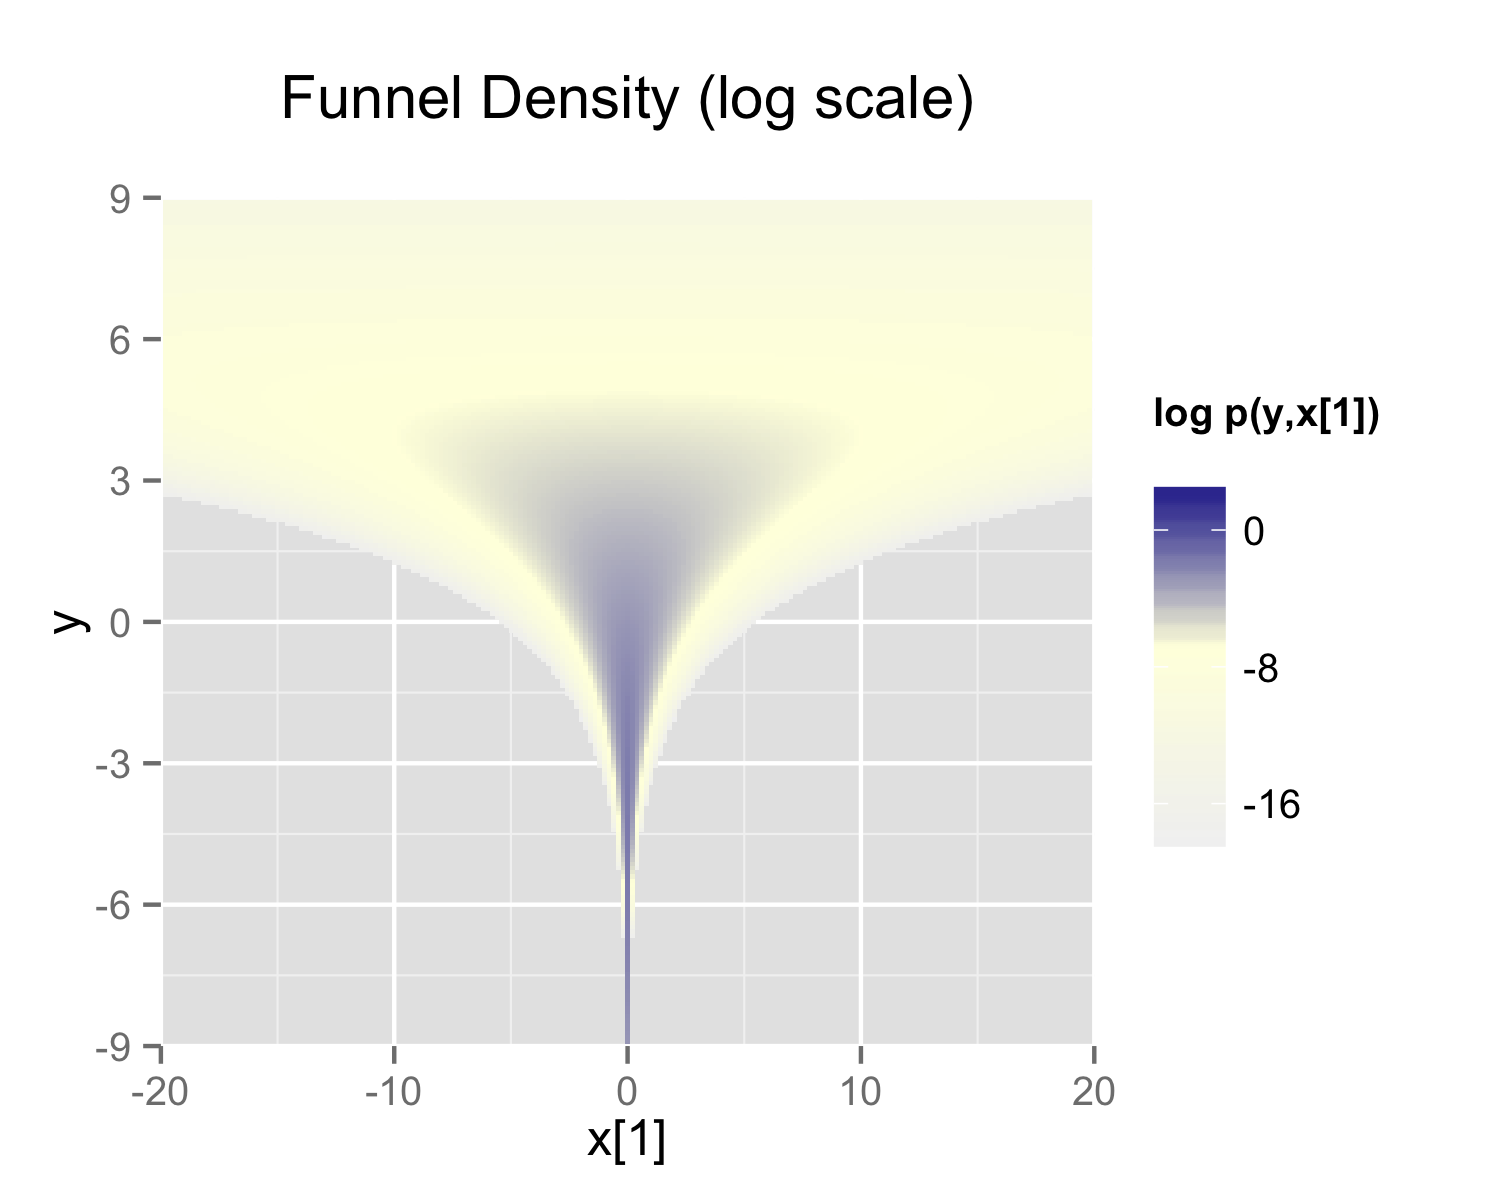
\includegraphics[height=2in]{img/funnel.png}
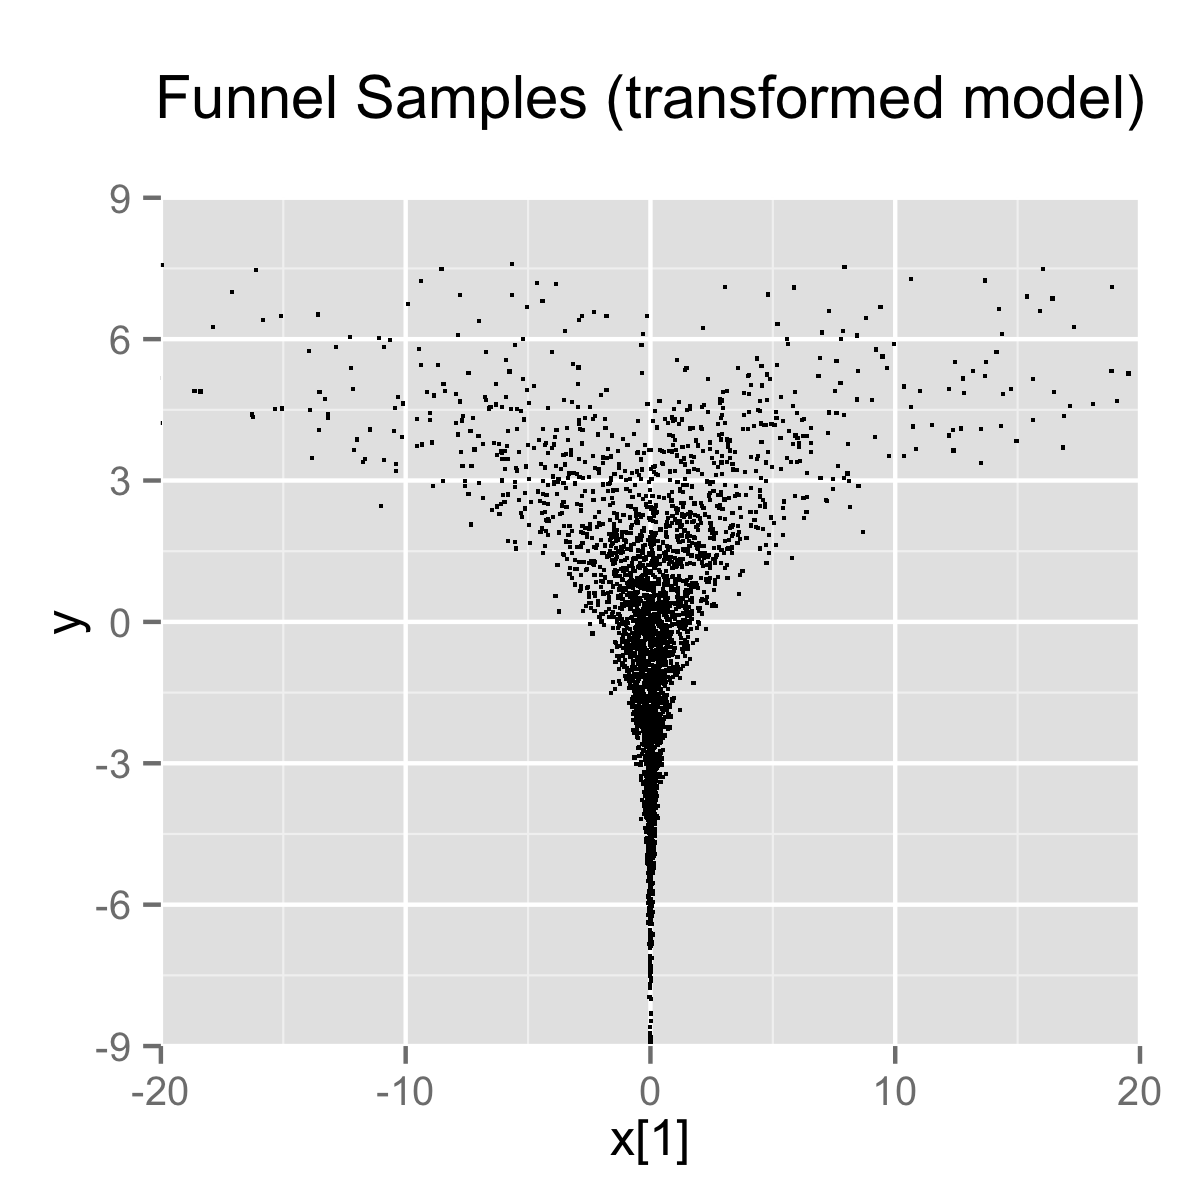
\includegraphics[height=2in]{img/funnel-fit.png}
\end{center}
\vspace*{-18pt}
\caption{\small\it Neal's Funnel.  (Left) The marginal density of
  Neal's funnel for the upper-level variable $y$ and one lower-level
  variable $x_1$ (see the text for the formula).  The blue region has
  log density greater than -8, the yellow region density greater than
  -16, and the gray background a density less than -16.
  (Right) 4000 draws from a run of Stan's
  sampler with default settings.  Both plots are restricted to the
  shown window of $x_1$ and $y$ values; some draws fell outside of
  the displayed area as would be expected given the density.  The samples are
  consistent with the marginal density $p(y) =
  \distro{Normal}(y|0,3)$, which has mean 0 and standard deviation
  3.}\label{funnel.figure}
\end{figure}

\citep{Neal:2003} defines a distribution that exemplifies the
difficulties of sampling from some hierarchical models.  Neal's
example is fairly extreme, but can be trivially reparameterized in
such a way as to make sampling straightforward.

Neal's example has support for $y \in
\mathbb{R}$ and  $x \in \mathbb{R}^9$ with density
%
\[
p(y,x) = \distro{Normal}(y|0,3) \times \prod_{n=1}^9
\distro{Normal}(x_n|0,\exp(y/2)).
\]
%
The probability contours are shaped like ten-dimensional funnels.  The
funnel's neck is particularly sharp because of the exponential
function applied to $y$.  A plot of the log marginal density of $y$
and the first dimension $x_1$ is shown in \reffigure{funnel}.

The funnel can be implemented directly in Stan as follows.
%
\begin{stancode}
parameters {
  real y;
  vector[9] x;
}
model {
  y ~ normal(0, 3);
  x ~ normal(0, exp(y/2));
}
\end{stancode}
%
When the model is expressed this way, Stan has trouble sampling from
the neck of the funnel, where $y$ is small and thus $x$ is constrained
to be near 0.  This is due to the fact that the density's scale
changes with $y$, so that a step size that works well in the body will
be too large for the neck and a step size that works in the neck will be
very inefficient in the body.

In this particular instance, because the analytic form of the density
from which samples are drawn is known, the model can be converted to
the following more efficient form.
%
\begin{stancode}
parameters {
  real y_raw;
  vector[9] x_raw;
}
transformed parameters {
  real y;
  vector[9] x;

  y = 3.0 * y_raw;
  x = exp(y/2) * x_raw;
}
model {
  y_raw ~ normal(0, 1); // implies y ~ normal(0, 3)
  x_raw ~ normal(0, 1); // implies x ~ normal(0, exp(y/2))
}
\end{stancode}
%
In this second model, the parameters \Verb|x_raw| and \Verb|y_raw| are
sampled as independent unit normals, which is easy for Stan.  These
are then transformed into samples from the funnel.  In this case, the
same transform may be used to define Monte Carlo samples directly
based on independent unit normal samples; Markov chain Monte Carlo
methods are not necessary. If such a reparameterization were used in
Stan code, it is useful to provide a comment indicating what the
distribution for the parameter implies for the distribution of the
transformed parameter.

\subsection{Reparameterizing the Cauchy}

Sampling from heavy tailed distributions such as the Cauchy is
difficult for Hamiltonian Monte Carlo, which operates within a
Euclidean geometry.%
%
\footnote{Riemannian Manifold Hamiltonian Monte Carlo (RMHMC) overcomes
  this difficulty by simulating the Hamiltonian dynamics in a space
  with a position-dependent metric; see
  \citep{GirolamiCalderhead:2011} and \citep{Betancourt:2012}.}
%
The practical problem is that tail of the Cauchy
requires a relatively large step size compared to the trunk.  With a
small step size, the No-U-Turn sampler requires many steps when
starting in the tail of the distribution; with a large step size,
there will be too much rejection in the central portion of the
distribution.  This problem may be mitigated by defining the
Cauchy-distributed variable as the transform of a uniformly
distributed variable using the Cauchy inverse cumulative distribution
function.

Suppose a random variable of interest $X$ has a Cauchy distribution
with location $\mu$ and scale $\tau$, so that $X \sim
\distro{Cauchy}(\mu,\tau)$.  The variable $X$ has a cumulative
distribution function $F_X:\reals \rightarrow (0,1)$ defined by
\[
F_X(x) = \frac{1}{\pi} \arctan \left( \frac{x - \mu}{\tau} \right) +
\frac{1}{2}.
\]
The inverse of the cumulative distribution function,
$F_X^{-1}:(0,1) \rightarrow \reals$, is thus
%
\[
F^{-1}_X(y) = \mu + \tau \tan \left( \pi \left( y - \frac{1}{2} \right) \right).
\]
Thus if the random variable $Y$ has a unit uniform distribution, $Y
\sim \distro{Uniform}(0,1)$, then $F^{-1}_X(Y)$ has a Cauchy
distribution with location $\mu$ and scale $\tau$, i.e., $F^{-1}_X(Y) \sim
\distro{Cauchy}(\mu,\tau)$.

Consider a Stan program involving a Cauchy-distributed parameter
\code{beta}.
%
\begin{stancode}
parameters {
  real beta;
  ...
}
model {
  beta ~ cauchy(mu, tau);
  ...
}
\end{stancode}
%
This declaration of \code{beta} as a parameter may be replaced with a
transformed parameter \code{beta} defined in terms of a
uniform-distributed parameter \code{beta\_unif}.
%
\begin{stancode}
parameters {
  real<lower=-pi()/2, upper=pi()/2> beta_unif;
  ...
}
transformed parameters {
  real beta;
  beta = mu + tau * tan(beta_unif);  // beta ~ cauchy(mu, tau)
}
model {
  beta_unif ~ uniform(-pi()/2, pi()/2);  // not necessary
  ...
}
\end{stancode}
%
It is more convenient in Stan to transform a uniform variable on
$(-\pi/2, \pi/2)$ than one on $(0,1)$.  The Cauchy location and scale
parameters, \code{mu} and \code{tau}, may be defined as data or may
themselves be parameters.  The variable \code{beta} could also be
defined as a local variable if it does not need to be included in the
sampler's output.

The uniform distribution on \code{beta\_unif} is defined explicitly in
the model block, but it could be safely removed from the program
without changing sampling behavior.  This is because $\log
\distro{Uniform}(\beta_{\mbox{\footnotesize unif}}|-\pi/2,\pi/2) =
-\log \pi$ is a constant and Stan only
needs the total log probability up to an additive constant.  Stan will spend
some time checking that that \code{beta\_unif} is between
\code{-pi()/2} and \code{pi()/2}, but this condition is guaranteed by
the constraints in the declaration of \code{beta\_unif}.

\subsection{Reparameterizing a Student-t Distribution}

One thing that sometimes works when you're having trouble with the
heavy-tailedness of Student-t distributions is to use the
gamma-mixture representation, which says that you can generate a
Student-t distributed variable $\beta$,
\[
\beta \sim \mbox{\sf Student-t}(\nu, 0, 1),
\]
by first generating a gamma-distributed precision (inverse variance)
$\tau$ according to
\[
\tau \sim \mbox{\sf Gamma}(\nu/2, \nu/2),
\]
and then generating $\beta$ from the normal distribution,
\[
\beta \sim \mbox{\sf Normal}(0,\tau^{-\frac{1}{2}}).
\]
%
Because $\tau$ is precision, $\tau^{-\frac{1}{2}}$ is the scale
(standard deviation), which is the parameterization used by Stan.

The marginal distribution of $\beta$ when you integrate out $\tau$ is
$\mbox{\sf Student-t}(\nu, 0, 1)$, i.e.,
\[
\mbox{\sf Student-t}(\beta | \nu,0,1).
=
\int_0^{\infty}
\,
\mbox{\sf Normal}(\beta | 0, 1 / \tau^{-\frac{1}{2}})
\times
\mbox{\sf Gamma}(\tau | \nu/2, \nu/2)
\
d\tau.
\]
%

To go one step further, instead of defining a $\beta$ drawn from a
normal with precision $\tau$, define $\alpha$ to be drawn from a unit
normal,
%
\[
\alpha \sim \mbox{\sf Normal}(0,1)
\]
%
and rescale by defining
%
\[
\beta = \alpha \, \tau^{-\frac{1}{2}}.
\]
%

Now suppose $\mu = \beta x$ is the product of $\beta$ with a
regression predictor $x$.  Then the reparameterization $\mu = \alpha
\tau^{-\frac{1}{2}} x$ has the same distribution, but in the original, direct
parameterization, $\beta$ has (potentially) heavy tails, whereas in
the second, neither $\tau$ nor $\alpha$ have heavy tails.

To translate into Stan notation, this reparameterization replaces
%
\begin{stancode}
parameters {
  real<lower=0> nu;
  real beta;
  ...
model {
  beta ~ student_t(nu, 0, 1);
  ...
\end{stancode}
%
with
%
\begin{stancode}
parameters {
  real<lower=0> nu;
  real<lower=0> tau;
  real alpha;
  ...
transformed parameters {
  real beta;
  beta = alpha / sqrt(tau);
  ...
model {
  real half_nu;
  half_nu = 0.5 * nu;
  tau ~ gamma(half_nu, half_nu);
  alpha ~ normal(0, 1);
  ...
\end{stancode}
%
Although set to \code{0} here, in most cases, the lower bound for the
degrees of freedom parameter \code{nu} can be set to \code{1} or
higher; when \code{nu} is 1, the result is a Cauchy distribution with
very fat tails and as \code{nu} approaches infinity, the Student-t
distribution approaches a normal distribution.  Thus the parameter
\code{nu} characterizes the heaviness of the tails of the model.

\subsection{Hierarchical Models and the Non-Centered Parameterization}

Unfortunately, the usual situation in applied Bayesian modeling
involves complex geometries and interactions that are not known
analytically.  Nevertheless, reparameterization can still be very
effective for separating parameters.

\subsubsection{Centered parameterization}

For example, a vectorized hierarchical model might draw a vector of
coefficients $\beta$ with definitions as follows.  The so-called
centered parameterization is as follows.
%
\begin{stancode}
parameters {
  real mu_beta;
  real<lower=0> sigma_beta;
  vector[K] beta;
  ...
model {
  beta ~ normal(mu_beta, sigma_beta);
  ...
\end{stancode}
%
Although not shown, a full model will have priors on both
\Verb|mu_beta| and \Verb|sigma_beta| along with data modeled based on
these coefficients.  For instance, a standard binary logistic
regression with data matrix \code{x} and binary outcome vector
\code{y} would include a likelihood statement such as form
\Verb|y ~ bernoulli_logit(x * beta)|, leading to an analytically
intractable posterior.

A hierarchical model such as the above will suffer from the same kind
of inefficiencies as Neal's funnel, because the values of \Verb|beta|,
\Verb|mu_beta| and \Verb|sigma_beta| are highly correlated in the
posterior.  The extremity of the correlation depends on the amount of
data, with Neal's funnel being the extreme with no data.  In these
cases, the non-centered parameterization, discussed in the next
section, is preferable; when there is a lot of data, the centered
parameterization is more efficient.  See
\cite{Betancourt-Girolami:2013} for more information on the effects of
centering in hierarchical models fit with Hamiltonian Monte Carlo.


\subsection{Non-Centered Parameterization}

Sometimes the group-level effects do not constrain the hierarchical
distribution tightly.  Examples arise when there is not many groups,
or when the inter-group variation is high.  In such cases,
hierarchical models can be made much more efficient by shifting the
data's correlation with the parameters to the hyperparameters. Similar
to the funnel example, this will be much more efficient in terms of
effective sample size when there is not much data (see
\citep{Betancourt-Girolami:2013}), and in more extreme cases will be
necessary to achieve convergence.
%
\begin{stancode}
parameters {
  vector[K] beta_raw;
  ...
transformed parameters {
  vector[K] beta;
  // implies: beta ~ normal(mu_beta, sigma_beta)
  beta = mu_beta + sigma_beta * beta_raw;
model {
  beta_raw ~ normal(0, 1);
  ...
\end{stancode}
%
Any priors defined for \Verb|mu_beta| and \Verb|sigma_beta| remain as
defined in the original model.

Reparameterization of hierarchical models is not limited to the normal
distribution, although the normal distribution is the best candidate
for doing so. In general, any distribution of parameters in the
location-scale family is a good candidate for reparameterization. Let
$\beta = l + s\alpha$ where $l$ is a location parameter and $s$ is a
scale parameter. Note that $l$ need not be the mean, $s$ need not
be the standard deviation, and neither the mean nor the standard
deviation need to exist. If $\alpha$ and $\beta$ are from the same
distributional family but $\alpha$ has location zero and unit scale,
while $\beta$ has location $l$ and scale $s$, then that distribution
is a location-scale distribution. Thus, if $\alpha$ were a parameter
and $\beta$ were a transformed parameter, then a prior distribution
from the location-scale family on $\alpha$ with location zero and unit
scale implies a prior distribution on $\beta$ with location $l$ and
scale $s$. Doing so would reduce the dependence between $\alpha$,
$l$, and $s$.

There are several univariate distributions in the location-scale
family, such as the Student t distribution, including its special
cases of the Cauchy distribution (with one degree of freedom) and the
normal distribution (with infinite degrees of freedom). As shown above,
if $\alpha$ is distributed standard normal, then $\beta$ is distributed
normal with mean $\mu = l$ and standard deviation $\sigma = s$. The
logistic, the double exponential, the generalized extreme value
distributions, and the stable distribution are also in the
location-scale family.

Also, if $z$ is distributed standard normal, then $z^2$ is distributed
chi-squared with one degree of freedom. By summing the squares of $K$
independent standard normal variates, one can obtain a single variate
that is distributed chi-squared with $K$ degrees of freedom. However,
for large $K$, the computational gains of this reparameterization may
be overwhelmed by the computational cost of specifying $K$ primitive
parameters just to obtain one transformed parameter to use in a model.



\subsection{Multivariate Reparameterizations}

The benefits of reparameterization are not limited to univariate
distributions. A parameter with a multivariate normal prior distribution
is also an excellent candidate for reparameterization. Suppose you intend
the prior for $\beta$ to be multivariate normal with mean vector $\mu$
and covariance matrix $\Sigma$. Such a belief is reflected by the
following code.
%
\begin{stancode}
data {
  int<lower=2> K;
  vector[K] mu;
  cov_matrix[K] Sigma;
  ...
parameters {
  vector[K] beta;
  ...
model {
  beta ~ multi_normal(mu, Sigma);
  ...
\end{stancode}
%
In this case \Verb|mu| and \Verb|Sigma| are fixed data, but they could
be unknown parameters, in which case their priors would be unaffected
by a reparameterization of \Verb|beta|.

If $\alpha$ has the same dimensions as $\beta$ but the elements of
$\alpha$ are independently and identically distributed standard normal
such that $\beta = \mu + L\alpha$, where $LL^\top = \Sigma$, then
$\beta$ is distributed multivariate normal with mean vector $\mu$ and
covariance matrix $\Sigma$. One choice for $L$ is the Cholesky factor
of $\Sigma$. Thus, the model above could be reparameterized as follows.
%
\begin{stancode}
data {
  int<lower=2> K;
  vector[K] mu;
  cov_matrix[K] Sigma;
  ...
transformed data {
  matrix[K, K] L;
  L = cholesky_decompose(Sigma);
}
parameters {
  vector[K] alpha;
  ...
transformed parameters {
  vector[K] beta;
  beta = mu + L * alpha;
}
model {
  alpha ~ normal(0, 1);
  // implies: beta ~ multi_normal(mu, Sigma)
  ...
\end{stancode}
%
This reparameterization is more efficient for two reasons. First, it
reduces dependence among the elements of \Verb|alpha| and second, it
avoids the need to invert \Verb|Sigma| every time \Verb|multi_normal|
is evaluated.

The Cholesky factor is also useful when a covariance matrix is
decomposed into a correlation matrix that is multiplied from both
sides by a diagonal matrix of standard deviations, where either the
standard deviations or the correlations are unknown parameters. The
Cholesky factor of the covariance matrix is equal to the product of
a diagonal matrix of standard deviations and the Cholesky factor of
the correlation matrix. Furthermore, the product of a diagonal matrix
of standard deviations and a vector is equal to the elementwise
product between the standard deviations and that vector. Thus, if for
example the correlation matrix \Verb|Tau| were fixed data but the
vector of standard deviations \Verb|sigma| were unknown parameters,
then a reparameterization of \Verb|beta| in terms of \Verb|alpha|
could be implemented as follows.
%
\begin{stancode}
data {
  int<lower=2> K;
  vector[K] mu;
  corr_matrix[K] Tau;
  ...
transformed data {
  matrix[K, K] L;
  L = cholesky_decompose(Tau);
}
parameters {
  vector[K] alpha;
  vector<lower=0>[K] sigma;
  ...
transformed parameters {
  vector[K] beta;
  // This equals mu + diag_matrix(sigma) * L * alpha;
  beta = mu + sigma .* (L * alpha);
}
model {
  sigma ~ cauchy(0, 5);
  alpha ~ normal(0, 1);
  // implies: beta ~ multi_normal(mu,
  //  diag_matrix(sigma) * L * L' * diag_matrix(sigma)))
  ...
\end{stancode}
%
This reparameterization of a multivariate normal distribution in
terms of standard normal variates can be extended to other multivariate
distributions that can be conceptualized as contaminations of the
multivariate normal, such as the multivariate Student t and the skew
multivariate normal distribution.

A Wishart distribution can also be reparameterized in terms of standard
normal variates and chi-squared variates. Let $L$ be the Cholesky factor
of a $K \times K$ positive definite scale matrix $S$ and let $\nu$ be
the degrees of freedom. If
%
\begin{equation*}
A = \left( \begin{array}{cccc}
\sqrt{c_{1}} & 0 & \cdots & 0\\
z_{21} & \sqrt{c_{2}} & \ddots & \vdots\\
\vdots & \ddots & \ddots & 0\\
z_{K1} & \cdots & z_{K\left(K-1\right)} & \sqrt{c_{K}}
 \end{array} \right),
\end{equation*}
%
where each $c_i$ is distributed chi-squared with $\nu - i + 1$ degrees
of freedom and each $z_{ij}$ is distributed standard normal, then
$W = LAA^{\top}L^{\top}$ is distributed Wishart with scale matrix
$S = LL^{\top}$ and degrees of freedom $\nu$. Such a reparameterization
can be implemented by the following Stan code:
%
\begin{stancode}
data {
  int<lower=1> N;
  int<lower=1> K;
  int<lower=K+2> nu
  matrix[K, K] L; // Cholesky factor of scale matrix
  vector[K] mu;
  matrix[N, K] y;
  ...
parameters {
  vector<lower=0>[K] c;
  vector[0.5 * K * (K - 1)] z;
  ...
model {
  matrix[K, K] A;
  int count = 1;
  for (j in 1:(K-1)) {
    for (i in (j+1):K) {
      A[i, j] = z[count];
      count += 1;
    }
    for (i in 1:(j - 1)) {
      A[i, j] = 0.0;
    }
    A[j, j] = sqrt(c[j]);
  }
  for (i in 1:(K-1))
    A[i, K] = 0;
  A[K, K] = sqrt(c[K]);

  for (i in 1:K)
    c[i] ~ chi_square(nu - i + 1);

  z ~ normal(0, 1);
  // implies: L * A * A' * L' ~ wishart(nu, L * L')
  y ~ multi_normal_cholesky(mu, L * A);
  ...
\end{stancode}
%
This reparameterization is more efficient for three reasons. First, it
reduces dependence among the elements of \Verb|z| and second, it
avoids the need to invert the covariance matrix, $W$ every time
\Verb|wishart| is evaluated. Third, if $W$ is to be used with a
multivariate normal distribution, you can pass $L A$ to the more
efficient \Verb|multi_normal_cholesky| function, rather than passing
$W$ to \Verb|multi_normal|.

If $W$ is distributed Wishart with scale matrix $S$ and degrees of
freedom $\nu$, then $W^{-1}$ is distributed inverse Wishart with inverse
scale matrix $S^{-1}$ and degrees of freedom $\nu$. Thus, the previous
result can be used to reparameterize the inverse Wishart distribution.
Since $W = L * A * A^{\top} * L^{\top}$,
$W^{-1} = L^{{\top}^{-1}} A^{{\top}^{-1}} A^{-1} L^{-1}$, where all four
inverses exist, but
$L^{{-1}^{\top}} = L^{{\top}^{-1}}$ and $A^{{-1}^{\top}} = A^{{\top}^{-1}}$.
We can slightly modify the above Stan code for this case:
%
\begin{stancode}
data {
  int<lower=1> K;
  int<lower=K+2> nu
  matrix[K, K] L; // Cholesky factor of scale matrix
  ...
transformed data {
  matrix[K, K] eye;
  matrix[K, K] L_inv;
  for (j in 1:K) {
    for (i in 1:K) {
      eye[i, j] = 0.0;
    }
    eye[j, j] = 1.0;
  }
  L_inv = mdivide_left_tri_low(L, eye);
}
parameters {
  vector<lower=0>[K] c;
  vector[0.5 * K * (K - 1)] z;
  ...
model {
  matrix[K, K] A;
  matrix[K, K] A_inv_L_inv;
  int count;
  count = 1;
  for (j in 1:(K-1)) {
    for (i in (j+1):K) {
      A[i, j] = z[count];
      count += 1;
    }
    for (i in 1:(j - 1)) {
      A[i, j] = 0.0;
    }
    A[j, j] = sqrt(c[j]);
  }
  for (i in 1:(K-1))
    A[i, K] = 0;
  A[K, K] = sqrt(c[K]);

  A_inv_L_inv = mdivide_left_tri_low(A, L_inv);
  for (i in 1:K)
    c[i] ~ chi_square(nu - i + 1);

  z ~ normal(0, 1); // implies: crossprod(A_inv_L_inv) ~
  // inv_wishart(nu, L_inv' * L_inv)
  ...
\end{stancode}
%
Another candidate for reparameterization is the Dirichlet distribution
with all $K$ shape parameters equal. \cite{ZyczkowskiSommers:2001} shows
that if $\theta_i$ is equal to the sum of $\beta$ independent squared
standard normal variates and $\rho_i = \frac{\theta_i}{\sum \theta_i}$,
then the $K$-vector $\rho$ is distributed Dirichlet with all shape
parameters equal to $\frac{\beta}{2}$. In particular, if $\beta = 2$,
then $\rho$ is uniformly distributed on the unit simplex. Thus, we can
make $\rho$ be a transformed parameter to reduce dependence, as in:
%
\begin{stancode}
data {
  int<lower=1> beta;
  ...
parameters {
  vector[beta] z[K];
  ...
transformed parameters {
  simplex[K] rho;
  for (k in 1:K)
    rho[k] = dot_self(z[k]); // sum-of-squares
  rho = rho / sum(rho);
}
model {
  for (k in 1:K)
    z[k] ~ normal(0, 1);
  // implies: rho ~ dirichlet(0.5 * beta * ones)
  ...
\end{stancode}
%

\section{Vectorization}

\subsection{Gradient Bottleneck}

Stan spends the vast majority of its time computing the gradient of
the log probability function, making gradients the obvious target for
optimization.  Stan's gradient calculations with algorithmic
differentiation require a template expression to be allocated%
%
\footnote{Stan uses its own arena-based allocation, so allocation and
  deallocation are faster than with a raw call to \code{new}.}
%
and constructed for each subexpression of a Stan program involving
parameters or transformed parameters.  This section defines
optimization strategies based on vectorizing these subexpressions to
reduce the work done during algorithmic differentiation.

\subsection{Vectorizing Summations}

Because of the gradient bottleneck described in the previous section,
it is more efficient to collect a sequence of summands into a vector
or array and then apply the \code{sum()} operation than it is to
continually increment a variable by assignment and addition.  For
example, consider the following code snippet, where \code{foo()} is
some operation that depends on \code{n}.
%
\begin{stancode}
for (n in 1:N)
  total += foo(n,...);
\end{stancode}
%
This code has to create intermediate representations for each
of the \code{N} summands.

A faster alternative is to copy the values into a vector, then
apply the \code{sum()} operator, as in the following refactoring.
%
\begin{stancode}
{
  vector[N] summands;
  for (n in 1:N)
    summands[n] = foo(n,...);
  total = sum(summands);
}
\end{stancode}
%
Syntactically, the replacement is a statement block delineated
by curly brackets (\Verb|{|, \Verb|}|), starting with the definition
of the local variable \code{summands}.

Even though it involves extra work to allocate the \code{summands}
vector and copy \code{N} values into it, the savings in
differentiation more than make up for it.  Perhaps surprisingly,
it will also use substantially less memory overall than incrementing
\code{total} within the loop.


\subsection{Vectorization through Matrix Operations}

The following program directly encodes a linear regression with fixed
unit noise using a two-dimensional array \code{x} of predictors, an
array \code{y} of outcomes, and an array \code{beta} of regression
coefficients.
%
\begin{stancode}
data {
  int<lower=1> K;
  int<lower=1> N;
  real x[K, N];
  real y[N];
}
parameters {
  real beta[K];
}
model {
  for (n in 1:N) {
    real gamma = 0;
    for (k in 1:K)
      gamma += x[n, k] * beta[k];
    y[n] ~ normal(gamma, 1);
  }
}
\end{stancode}
%
The following model computes the same log probability function as the
previous model, even supporting the same input files for data and
initialization.
%
\begin{stancode}
data {
  int<lower=1> K;
  int<lower=1> N;
  vector[K] x[N];
  real y[N];
}
parameters {
  vector[K] beta;
}
model {
  for (n in 1:N)
    y[n] ~ normal(dot_product(x[n], beta), 1);
}
\end{stancode}
%
Although it produces equivalent results, the dot product should not be
replaced with a transpose and multiply, as in
%
\begin{stancode}
        y[n] ~ normal(x[n]' * beta, 1);
\end{stancode}
%
The relative inefficiency of the transpose and multiply approach is
that the transposition operator allocates a new vector into which the
result of the transposition is copied.  This consumes both time
and memory%
%
\footnote{Future versions of Stan may remove this inefficiency by more
  fully exploiting expression templates inside the Eigen \Cpp matrix
  library.  This will require enhancing Eigen to deal with mixed-type
  arguments, such as the type \code{double} used for constants and the
  algorithmic differentiation type \code{stan::math::var} used for
  variables.}.
%
The inefficiency of transposition could itself be mitigated somewhat by
reordering the product and pulling the transposition out of the loop,
as follows.
%
\begin{stancode}
...
transformed parameters {
  row_vector[K] beta_t;
  beta_t = beta';
}
model {
  for (n in 1:N)
    y[n] ~ normal(beta_t * x[n], 1);
}
\end{stancode}
%
The problem with transposition could be completely solved by directly
encoding the \code{x} as a row vector, as in the
following example.
%
\begin{stancode}
data {
  ...
  row_vector[K] x[N];
  ...
}
parameters {
  vector[K] beta;
}
model {
  for (n in 1:N)
    y[n] ~ normal(x[n] * beta, 1);
}
\end{stancode}
%
Declaring the data as a matrix and then computing all the predictors
at once using matrix multiplication is more efficient still, as in the
example discussed in the next section.

Having said all this, the most efficient way to code this model is
with direct matrix multiplication, as in
%
\begin{stancode}
data {
  matrix[N, K] x;
  vector[N] y;
}
parameters {
  vector[K] beta;
}
model {
  y ~ normal(x * beta, 1);
\end{stancode}
%
In general, encapsulated single operations that do the work of loops
will be more efficient in their encapsulated forms.  Rather than
performing a sequence of row-vector/vector multipliations, it is
better to encapsulate it as a single matrix/vector multiplication.

\subsection{Vectorized Probability Functions}

The final and most efficient version replaces the loops and
transformed parameters by using the vectorized form of the normal
probability function, as in the following example.
%
\begin{stancode}
data {
  int<lower=1> K;
  int<lower=1> N;
  matrix[N, K] x;
  vector[N] y;
}
parameters {
  vector[K] beta;
}
model {
  y ~ normal(x * beta, 1);
}
\end{stancode}
%
The variables are all declared as either matrix or vector types.
The result of the matrix-vector multiplication \code{x * beta} in the
model block is a vector of the same length as \code{y}.

The probability function documentation in \refpart{built-in-functions}
indicates which of Stan's probability functions support
vectorization; see \refsection{prob-vectorization} for more
information.  Vectorized probability functions accept either vector or
scalar inputs for all arguments, with the only restriction being that
all vector arguments are the same dimensionality.  In the example
above, \code{y} is a vector of size \code{N}, \code{x * beta} is a
vector of size \code{N}, and \code{1} is a scalar.

\subsection{Reshaping Data for Vectorization}

Sometimes data does not arrive in a shape that is ideal for
vectorization, but can be put into such shape with some munging
(either inside Stan's transformed data block or outside).

John Hall provided a simple example on the Stan users group.
Simplifying notation a bit, the original model had a sampling
statement in a loop, as follows.
%
\begin{stancode}
for (n in 1:N)
  y[n] ~ normal(mu[ii[n]], sigma);
\end{stancode}
%
The brute force vectorization would build up a mean vector and then
vectorize all at once.
%
\begin{stancode}
{
  vector[N] mu_ii;
  for (n in 1:N)
    mu_ii[n] = mu[ii[n]];
  y ~ normal(mu_ii, sigma);
\end{stancode}
%
If there aren't many levels (values \code{ii[n]} can take), then it
behooves us to reorganize the data by group in a case like this.
Rather than having a single observation vector \code{y}, there are K of them.
And because Stan doesn't support ragged arrays, it means K
declarations.  For instance, with 5 levels, we have
%
\begin{stancode}
  y_1 ~ normal(mu[1], sigma);
  ...
  y_5 ~ normal(mu[5], sigma);
\end{stancode}
%
This way, both the \code{mu} and \code{sigma} parameters are shared.
Which way works out to be more efficient will depend on the shape of
the data; if the sizes are very small, the simple vectorization may be
faster, but for moderate to large sized groups, the full expansion
should be faster.

\section{Exploiting Sufficient Statistics}

In some cases, models can be recoded to exploit sufficient statistics
in estimation.  This can lead to large efficiency gains compared to an
expanded model.  For example, consider the following Bernoulli
sampling model.
%
\begin{stancode}
data {
  int<lower=0> N;
  int<lower=0, upper=1> y[N];
  real<lower=0> alpha;
  real<lower=0> beta;
}
parameters {
  real<lower=0, upper=1> theta;
}
model {
  theta ~ beta(alpha, beta);
  for (n in 1:N)
    y[n] ~ bernoulli(theta);
}
\end{stancode}
%
In this model, the sum of positive outcomes in \code{y} is a
sufficient statistic for the chance of success \code{theta}.  The
model may be recoded using the binomial distribution as follows.
%
\begin{stancode}
    theta ~ beta(alpha, beta);
    sum(y) ~ binomial(N, theta);
\end{stancode}
%
Because truth is represented as one and falsehood as zero, the sum
\code{sum(y)} of a binary vector \code{y} is equal to the number of
positive outcomes out of a total of \code{N} trials.

This can be generalized to other discrete cases (one wouldn't expect
continuous observations to be duplicated if they are random).  Suppose
there are only $K$ possible discrete outcomes, $z_1, \ldots, z_K$, but
there are $N$ observations, where $N$ is much larger than $K$.  If
$f_k$ is the frequency of outcome $z_k$, then the entire likelihood
with distribution \code{foo} can be coded as follows.
%
\begin{stancode}
for (k in 1:K)
  target += f[k] * foo_lpmf(z[k] | ...);
\end{stancode}
%
where the ellipses are the parameters of the log probability mass
function for distribution \code{foo} (there's no distribution called
``foo''; this is just a placeholder for any discrete distribution
name).

The resulting program looks like a ``weighted'' regression, but here
the weights \code{f[k]} are counts and thus sufficient statistics for
the pmf and simply amount to an alternative, more efficient coding of
the same likelihood.  For efficiency, the frequencies \code{f[k]}
should be counted once in the transformed data block and stored.


\section{Aggregating Common Subexpressions}

If an expression is calculated once, the value should be saved and
reused wherever possible.  That is, rather than using
\code{exp(theta)} in multiple places, declare a local variable to
store its value and reuse the local variable.

Another case that may not be so obvious is with two multilevel
parameters, say \code{a[ii[n]] + b[jj[n]]}.  If \code{a} and \code{b}
are small (i.e., do not have many levels), then a table \code{a\_b} of
their sums can be created, with
%
\begin{stancode}
matrix[size(a), size(b)] a_b;
for (i in 1:size(a))
  for (j in 1:size(b))
    a_b[i, j] = a[i] + b[j];
\end{stancode}
%
Then the sum can be replaced with \code{a\_b[ii[n], jj[n]]}.


\section{Exploiting Conjugacy}


Continuing the model from the previous section, the conjugacy of the
beta prior and binomial sampling distribution allow the model to be
further optimized to the following equivalent form.
%
\begin{stancode}
    theta ~ beta(alpha + sum(y), beta + N - sum(y));
\end{stancode}
%
To make the model even more efficient, a transformed data variable
defined to be \code{sum(y)} could be used in the place of \code{sum(y)}.

\section{Standardizing Predictors and Outputs}

Stan programs will run faster if the input is standardized to have a
zero sample mean and unit sample variance.  This section illustrates
the principle with a simple linear regression.

Suppose that $y = (y_1,\ldots,y_N)$ is a sequence of $N$ outcomes and
$x = (x_1,\ldots,x_N)$ a parallel sequence of $N$ predictors.  A
simple linear regression involving an intercept coefficient $\alpha$
and slope coefficient $\beta$ can be expressed as
\[
y_n = \alpha + \beta x_n + \epsilon_n,
\]
where
\[
\epsilon_n \sim \distro{Normal}(0,\sigma).
\]

If either vector $x$ or $y$ has very large or very small values or if the
sample mean of the values is far away from 0 (on the scale of the values),
then it can be more efficient to standardize the outputs $y_n$ and
predictors $x_n$.  The data is first centered by subtracting the
sample mean, and then scaled by dividing by the sample deviation.
Thus a data point $u$ is standardized with respect to
a vector $y$  by the function $\mbox{z}_y$, defined by
\[
\mbox{z}_y(u) = \frac{u - \bar{y}}{\mbox{sd}(y)}
\]
where the sample mean of $y$ is
\[
\bar{y}
= \frac{1}{N} \sum_{n=1}^N y_n,
\]
and the sample standard deviation of $y$ is
\[
\mbox{sd}(y)
= \left(
\frac{1}{N} \sum_{n=1}^N (y_n - \bar{y})^2
\right)^{1/2}.
\]
The inverse transform is
defined by reversing the two normalization steps, first rescaling by
the same deviation and relocating by the sample mean,
\[
\mbox{z}_y^{-1}(v) = \mbox{sd}(y) v + \bar{y}.
\]

To standardize a regression problem, the predictors and outcomes are
standardized.  This changes the scale of the variables, and hence
changes the scale of the priors.  Consider the following initial
model.
%
\begin{stancode}
data {
  int<lower=0> N;
  vector[N] y;
  vector[N] x;
}
parameters {
  real alpha;
  real beta;
  real<lower=0> sigma;
}
model {
  // priors
  alpha ~ normal(0, 10);
  beta ~ normal(0, 10);
  sigma ~ cauchy(0, 5);
  // likelihood
  for (n in 1:N)
    y[n] ~ normal(alpha + beta * x[n], sigma);
}
\end{stancode}
%

The data block for the standardized model is identical.  The
standardized predictors and outputs are defined in the transformed
data block.
%
\begin{stancode}
data {
  int<lower=0> N;
  vector[N] y;
  vector[N] x;
}
transformed data {
  vector[N] x_std;
  vector[N] y_std;
  x_std = (x - mean(x)) / sd(x);
  y_std = (y - mean(y)) / sd(y);
}
parameters {
  real alpha_std;
  real beta_std;
  real<lower=0> sigma_std;
}
model {
  alpha_std ~ normal(0, 10);
  beta_std ~ normal(0, 10);
  sigma_std ~ cauchy(0, 5);
  for (n in 1:N)
    y_std[n] ~ normal(alpha_std + beta_std * x_std[n],
                      sigma_std);
}
\end{stancode}
%
The parameters are renamed to indicate that they aren't the
``natural'' parameters, but the model is otherwise identical.  In
particular, the fairly diffuse priors on the coefficients and error
scale are the same.  These could have been transformed as well, but
here they are left as is, because the scales make sense as very
diffuse priors for standardized data; the priors could be made more
informative.  For instance, because the outputs $y$ have been
standardized, the error $\sigma$ should not be greater than 1, because
that's the scale of the noise for predictors $\alpha = \beta = 0$.

The original regression
\[
y_n
= \alpha + \beta x_n + \epsilon_n
\]
has been transformed to a regression on the standardized variables,
\[
\mbox{z}_y(y_n)
= \alpha'
+ \beta' \mbox{z}_x(x_n)
+ \epsilon'_n.
\]
The original parameters can be recovered with a little algebra,
%
\begin{eqnarray*}
y_n
& = & \mbox{z}_y^{-1}(\mbox{z}_y(y_n))
\\[4pt]
& = &
\mbox{z}_y^{-1}
\left(
\alpha'
+ \beta' \mbox{z}_x(x_n)
+ \epsilon_n'
\right)
\\[4pt]
& = &
\mbox{z}_y^{-1}
\left(
\alpha'
+ \beta'
    \left(
      \frac{x_n - \bar{x}}{\mbox{\small sd}(x)}
    \right)
+ \epsilon_n'
\right)
\\[4pt]
& = &
\mbox{sd}(y)
\left(
\alpha'
+ \beta'
    \left(
      \frac{x_n - \bar{x}}{\mbox{\small sd}(x)}
    \right)
+ \epsilon_n'
\right)
+ \bar{y}
\\[4pt]
& = &
\left(
  \mbox{sd}(y)
      \left(
          \alpha'
          - \beta' \frac{\bar{x}}{\mbox{\small sd}(x)}
      \right)
  + \bar{y}
\right)
+ \left(
      \beta' \frac{\mbox{\small sd}(y)}{\mbox{\small sd}(x)}
  \right) x_n
+ \mbox{sd}(y) \epsilon'_n,
\end{eqnarray*}
%
from which the original scale parameter values can be read off,
\[
\alpha
=
\mbox{sd}(y)
      \left(
          \alpha'
          - \beta' \frac{\bar{x}}{\mbox{\small sd}(x)}
      \right)
  + \bar{y};
\ \ \ \ \
\beta = \beta' \frac{\mbox{\small sd}(y)}{\mbox{\small sd}(x)};
\ \ \ \ \
\sigma = \mbox{sd}(y) \sigma'.
\]
%
These recovered parameter values on the original scales can be
calculated within Stan using a generated quantities block following
the model block,
\begin{stancode}
generated quantities {
  real alpha;
  real beta;
  real<lower=0> sigma;
  alpha = sd(y) * (alpha_std - beta_std * mean(x) / sd(x))
           + mean(y);
  beta = beta_std * sd(y) / sd(x);
  sigma = sd(y) * sigma_std;
}
\end{stancode}
%
Of course, it is inefficient to compute all of the means and standard
deviations every iteration; for more efficiency, these can be
calculated once and stored as transformed data.  Furthermore, the
model sampling statement can be easily vectorized, for instance, in
the transformed model, to
\begin{stancode}
    y_std ~ normal(alpha_std + beta_std * x_std, sigma_std);
\end{stancode}
